% ===========================================================================
%  Paper A -- Negative reflection of guided waves at a free edge in a
%  flexoelectric piezoelectric-semiconductor plate: the strain-gradient
%  backward branch
%
%  Build:  pdflatex main && bibtex main && pdflatex main && pdflatex main
%
%  NOTE ON THE BUILD TEST.  The authoring environment used for the final
%  correction had no TeX installation available, so the source below was
%  validated statically (balanced environments, every \cite key resolved
%  against references.bib, every \ref matched to a \label, every figure file
%  present, no undefined macros) but was NOT compiled.  See the round-4
%  report PAPER_A_FINAL_SCIENTIFIC_AUDIT.md, section 11.
% ===========================================================================
\documentclass[10pt,a4paper]{article}

\usepackage[margin=22mm]{geometry}
\usepackage[T1]{fontenc}
\usepackage{lmodern}
\usepackage{amsmath}
\usepackage{amssymb}
\usepackage{mathtools}
\usepackage{siunitx}
\usepackage{graphicx}
\usepackage{booktabs}
\usepackage{tabularx}
\usepackage[font=small,labelfont=bf]{caption}
\usepackage{subcaption}
\usepackage[hidelinks]{hyperref}
\usepackage{cleveref}

% siunitx v2 and v3 both understand \sisetup.  The previous source used
% \siunitxsetup, which exists only in v3 and aborted the build on v2.
\sisetup{detect-all=true,per-mode=symbol,exponent-product=\times,
         group-separator={,},group-minimum-digits=4}

% Line-breaking slack for the prose.  This absorbs the residual overfull lines
% of long inline paths and wide math without touching the font size anywhere.
\setlength{\emergencystretch}{2em}

% amsmath already defines \boldsymbol; the previous source redefined it with
% \newcommand, which is a hard "already defined" error.  The definition below
% only introduces a short alias and leaves \boldsymbol untouched.
\newcommand{\vect}[1]{\boldsymbol{#1}}
\newcommand{\dd}{\mathrm{d}}
\newcommand{\ii}{\mathrm{i}}
\newcommand{\ee}{\mathrm{e}}
\DeclareMathOperator{\Real}{Re}
\DeclareMathOperator{\Imag}{Im}

\title{\bfseries Backward-branch negative reflection of guided waves at a free
edge in a flexoelectric piezoelectric--semiconductor plate}

\author{Vipin Kumar\textsuperscript{*}\\[2pt]
\small Department of Applied Mechanics, Indian Institute of Technology Delhi,
New Delhi 110016, India}

\date{\today}

\begin{document}
\maketitle

\begin{abstract}
\noindent
Strain gradients polarise a dielectric, and in a piezoelectric semiconductor the
resulting polarisation is screened by mobile carriers; whether that coupling
alters the way a guided plate mode is scattered at a free edge has not been
settled.  A transversely isotropic ($6mm$) n-type ZnO plate of thickness $d$ is
modelled with strain-gradient elasticity, piezoelectricity, flexoelectricity and
linearised electron drift--diffusion, the only constitutive addition being a
bilinear carrier--strain-gradient enthalpy, and the free-edge problem is solved
as a Fourier-reduced spectral Galerkin matching of outgoing modes.  At
$k_xd=0.736$ (\SI{16.68}{\giga\hertz}) the backward-propagating branch carries
\SI{2.31}{\percent} of the incident power; along the same branch the share rises
to a maximum of \SI{94.68}{\percent} at $k_xd=0.5275$
(\SI{16.6547}{\giga\hertz}), where the incident and backward wavenumbers differ
by \SI{0.4}{\percent} and the group velocity is below
\SI{1}{\metre\per\second}.  The maximum is a certified local extremum, flat to
\SI{0.01}{} percentage point over $0.5266\le k_xd\le0.5277$, and a modal share:
\SI{99.77}{\percent} of the incident power leaves as propagating modes, although
the incident flux at the fold is a factor 128 smaller than at the operating
point.  Removing
the strain-gradient sector removes the backward branch, while switching the
coupling off leaves the share unchanged; at its tabulated extreme the coupling
lowers the share by \SI{1.21}{\percent} at the operating point and by
\SI{34.2}{\percent} at the maximum, chiefly by attenuating the backward mode.
The gradient length, flexoelectric coefficient and coupling are synthetic;
corner line forces are not certified.

\medskip
\noindent\textbf{Keywords:} flexoelectricity; piezoelectric semiconductor;
strain-gradient elasticity; guided waves; negative reflection; spectral Galerkin
method.
\end{abstract}

\section{Introduction}
\label{sec:intro}

The classical theory of piezoelectricity relates the electric displacement to
the strain and the electric field alone.  Flexoelectricity adds a dependence on
the \emph{gradient} of strain \cite{shen2010theory,deng2020impact}, so that a
bending deformation polarises a dielectric even when it is centrosymmetric and
carries no piezoelectric constant.  The effect is small in absolute terms but
it scales as the inverse of a length, and it therefore becomes competitive with
piezoelectricity in thin films, at free surfaces and around edges and cracks,
where the strain gradient is large.  In a semiconductor the polarisation is not
merely a passive consequence of deformation: the induced bound charge is
screened by the mobile carrier gas, the screening redistributes the carriers,
and the redistribution feeds back on the electric field.  This closed loop --
strain gradient $\rightarrow$ polarisation $\rightarrow$ carrier redistribution
$\rightarrow$ field $\rightarrow$ strain -- is the subject of the rapidly
developing theory of flexoelectric semiconductors
\cite{qu2020mobile,qu2022thermal}.

Two strands of that literature are directly relevant here.  The first is the
continuum formulation itself.  Starting from a free-energy density that contains
the strain, the strain gradient, the electric field and the carrier
concentration perturbation, one obtains the field equations by independent
variations with respect to the displacement, the potential and the carrier
density.  Qu, Jin and Yang \cite{qu2020mobile} used this route to show that the
mechanical field redistributes mobile charge in a composite flexoelectric
dielectric--semiconductor beam, Qu, Jin and Yang \cite{qu2022bending} carried the same construction to the
bending of a flexoelectric semiconductor plate, and Qu, Zhang, Gao and Jin
\cite{qu2022thermal} extended the model to thermally induced carrier
redistribution, where the temperature gradient acts as an additional driving
term for the charge.  The most complete statement of the framework is the
Coleman--Noll derivation of Qu, Pan, Zhu and Deng \cite{qu2025thermodynamic},
whose additive free-energy decomposition is the reference against which the
added term of \cref{sec:intro_coupling} is placed in
\cref{sec:disc_literature}.  All these works make the point that must be respected in any
subsequent extension: the extra constitutive couplings are not free parameters
of a model, they are constrained by a thermodynamic potential, and the
reciprocal partner of every added term in the stress must appear in the
electrochemical potential.

The second strand is the wave theory.  Yang, Deng, Liang and Shen
\cite{yang2018lamb} derived the dispersion of Lamb waves in a plate with both
flexoelectricity and strain-gradient elasticity, and Yang, Liang, Deng and Shen
\cite{yang2020rayleigh} treated Rayleigh waves on a centrosymmetric
flexoelectric half-space.  Wang, Zhang, Zhang, Du, Xiao and Lou
\cite{wang2025rayleigh} recently combined both effects with the carrier physics
of a piezoelectric semiconductor layer on an elastic substrate and showed that
the layer thickness, the steady carrier concentration and the bias field all
move the dispersion and the attenuation of the surface wave.  Biswas and Sahu \cite{biswas2025rayleigh} extended the
half-space treatment to an n-type flexoelectric piezoelectric semiconductor with
second-order strain gradients and reported how the flexoelectric coefficients and
the steady carrier concentration move the Rayleigh velocity of that structure.
Zhang, Zhao, Hu,
Nie and Liu \cite{zhang2025pscplate} gave an exact Stroh-type treatment of a
piezoelectric semiconductor plate and identified the range of carrier
concentrations in which the semiconductor coupling is active at all -- outside
that range the plate reverts to a piezoelectric or even a purely elastic
behaviour.  These studies establish three facts that frame the present work:
flexoelectric and strain-gradient terms change the dispersion of guided modes;
the carrier physics is active only inside a window of doping; and the
attenuation of a guided mode can be controlled by the electrical boundary
conditions rather than by the mechanical ones.

What has not been examined in that literature is the \emph{scattering} problem
at an edge of a guided plate.  Reflection at a free surface of a flexoelectric
medium has been treated for plane waves in a half-space, where the result is a
set of reflection coefficients for the few body waves that the half-space
supports \cite{mondal2022scattering}; the modal partition of a \emph{guided}
plate branch at an edge, where the outgoing spectrum is discrete and contains a
backward-propagating member, and where the carriers participate in the
partition, has not been computed.  A guided mode that travels towards a free
edge has to convert into the set of outgoing modes that the edge can support.  In a purely elastic plate
this is a classical problem: an incident mode is reflected into its time-reverse
partner and into a finite family of mode-converted branches, and a
backward-propagating branch --- one whose energy flux opposes its phase
velocity --- can be excited whenever the edge problem admits such a branch.  We
therefore ask two questions and answer them separately.  Does this plate admit a
backward branch at the reported frequency, and how strongly does the edge
convert into it?  And does the carrier--strain-gradient coupling bias that
partition?  The answers turn out to be different in kind: the branch, and
therefore the strong conversion, is supplied by the strain-gradient sector
alone, while the added coupling only modifies it --- by one per cent at the
operating point, and by a third at the certified maximum through the extra
attenuation it gives the backward mode.  Reporting the two separately, rather
than attributing the effect to the new term, is what the rest of the paper
does.

\subsection{The added coupling and its reciprocals}
\label{sec:intro_coupling}

The model used here is deliberately minimal.  On top of the standard
flexoelectric piezoelectric-semiconductor enthalpy we add a single bilinear
term,
\begin{equation}
\label{eq:added_coupling}
\Delta\mathcal{H}=\Delta n\,H_{jkl}\,\varepsilon_{jk,l},
\end{equation}
where $\Delta n$ is the carrier-concentration perturbation, $\varepsilon_{jk,l}$
the strain gradient and $H_{jkl}$ a third-order coupling tensor with the units
of energy times length.  Because the enthalpy is a thermodynamic potential, the
term in \cref{eq:added_coupling} generates two partners.  Differentiating with
respect to the strain gradient gives an addition to the higher-order
(hyper)stress,
\begin{equation}
\label{eq:added_hyperstress}
\Delta\tau_{jkl}=\frac{\partial\Delta\mathcal{H}}{\partial\varepsilon_{jk,l}}
=H_{jkl}\,\Delta n,
\end{equation}
and differentiating with respect to the carrier density gives an addition to the
electrochemical potential,
\begin{equation}
\label{eq:added_mu}
\Delta\widetilde\mu=\frac{\partial\Delta\mathcal{H}}{\partial\Delta n}
=H_{jkl}\,\varepsilon_{jk,l}.
\end{equation}
Equations \eqref{eq:added_coupling}--\eqref{eq:added_mu} are one assumption,
not three.  They are the only new physics in the paper.  No additional field,
no micro-inertia, no flexoelectric-gradient term and no nonlinear
electromechanical feedback is introduced, and the classical constants are not
refitted.

The reciprocal relation \eqref{eq:added_mu} is what makes the edge problem
interesting.  A guided plate mode carries a strain gradient through the
thickness, so it perturbs the electrochemical potential even before any carrier
moves; the carriers respond, the charge density changes, and the changed charge
density modifies the hyperstress through \eqref{eq:added_hyperstress}.  The loop
is closed at the edge, where the conversion into outgoing branches takes place.

\subsection{Scope and organisation}
\label{sec:intro_scope}

The paper is organised as follows.  \Cref{sec:governing} states the
variational principle, the constitutive relations, the field equations and the
boundary conditions, and fixes the nomenclature for the plate surfaces, the
reflecting edge, the mechanical tractions, the higher-order double tractions,
the electrical conditions and the carrier-blocking conditions.
\Cref{sec:numerics} describes the solution strategy: a Fourier reduction in the
tangential direction with a single conserved wavenumber $k_y$, a spectral
Galerkin discretisation through the thickness, a companion-matrix formulation
in the direction of propagation, and an edge-matching step that separates
incoming from outgoing modes.
\Cref{sec:results} presents the ten figures of the study and, for each, states
what the panel is allowed to claim.  \Cref{sec:discussion} discusses what the
numbers mean and, at least as importantly, what they do not mean.
\Cref{sec:conclusions} lists the limitations that we could not remove.

Three conventions are used throughout and are worth stating once.  The plate
occupies $x<0$ and the reflecting edge is at $x=0$; the $z$ axis is the
six-fold axis of ZnO and points through the thickness, with the faces at
$z=\pm d/2$.  A quantity is called \emph{backward} when its energy flux has a
negative component along $x$, which is the direction of propagation of the
incident wave.  A mode is called \emph{outgoing} when it either decays away
from the edge or, if it is propagating, carries energy away from the edge.
All three definitions are operational: they are the ones implemented in the
solver, not merely the ones used in the prose.

\section{Mathematical formulation}
\label{sec:governing}

The formulation is built in the order in which the constitutive statement
generates the equations of motion: the geometry and the fields are fixed first
(\cref{sec:governing_variational}), then the kinematics and the gradient energy
(\cref{sec:governing_kinematics}), then the enthalpy from which every
constitutive relation is differentiated (\cref{sec:governing_constitutive}),
then the balance laws obtained by independent variations
(\cref{sec:governing_balance}), then the electric model with the two ratios
that justify it (\cref{sec:governing_electric}), the boundary conditions
(\cref{sec:governing_bc}), the power flux that defines a backward mode
(\cref{sec:governing_energy}), the dimensionless groups
(\cref{sec:governing_nondim}), the limits of the model
(\cref{sec:governing_limits}) and the condition under which the enthalpy stays
positive definite (\cref{sec:governing_stability}).

\subsection{Geometry, fields and notation}
\label{sec:governing_variational}

Consider a transversely isotropic ($6mm$) n-type ZnO plate of thickness $d$
whose faces are the planes $z=\pm d/2$, occupying the half-space $x<0$ and
terminating at a traction-free edge at $x=0$.  The plate is unbounded in $y$, so
a single tangential wavenumber $k_y$ is conserved, and every field has the form
$f(x,z)\,e^{ik_yy-i\omega t}$ with three displacement components retained.  The
formulation is therefore two-and-a-half-dimensional (2.5D): a discrete
cross-section in $(x,z)$ carrying full three-component kinematics, a single
conserved tangential wavenumber, and no discretisation of $y$.  The independent fields are
the displacement $u_i(\vect{x},t)$, the electrostatic potential
$\varphi(\vect{x},t)$ and the electron-number perturbation
$\Delta n(\vect{x},t)$ measured from the uniform doping $n_0$.  The polar $c$
axis of the crystal is $x_3\equiv z$; Latin indices run over $1,2,3$, a comma
denotes a spatial derivative and a superimposed dot a time derivative.

Three conventions are fixed once and used everywhere.  The electric field is
$E_i=-\partial_i\varphi$.  The electron charge is $-q$ with $q>0$.  The
quantity $\widetilde\mu$ is the \emph{electrochemical potential of an electron
per carrier}, measured in joules, so that every term appearing in it is an
energy and no term is a dimensionless ratio.

\subsection{Kinematics and the strain gradient}
\label{sec:governing_kinematics}

The small-strain tensor and its gradient are
\begin{equation}
\label{eq:strain}
\varepsilon_{ij}=\tfrac12\bigl(u_{i,j}+u_{j,i}\bigr),
\qquad
\eta_{ijk}\equiv\varepsilon_{ij,k}=\tfrac12\bigl(u_{i,jk}+u_{j,ik}\bigr),
\end{equation}
so that $\eta_{ijk}$ is symmetric in its first two indices,
$\eta_{ijk}=\eta_{jik}$, and carries the dimension of an inverse length.
All three displacement components are retained; the strain has six independent
components and the strain gradient eighteen.

The higher-order elastic energy is taken in the single-length
(isotropic-gradient) form
\begin{equation}
\label{eq:gradient_energy}
w_g=\tfrac12\,A_{ijklmn}\,\eta_{ijk}\,\eta_{lmn}
=\tfrac12\,\ell^{2}\,c_{ijlm}\,\eta_{ijk}\,\eta_{lmk},
\qquad
A_{ijklmn}=\ell^{2}\,c_{ijlm}\,\delta_{kn},
\end{equation}
where in \eqref{eq:gradient_energy} the \emph{third and sixth slots} of
$A_{ijklmn}$ are the gradient directions: the third slot is contracted with the
gradient index of the first strain gradient and the sixth with that of the
second.  This is the only contraction for which the energy depends on the
gradient of the strain through $c_{ijlm}\eta_{ijk}\eta_{lmk}$; contracting any
other pair of slots would break the major symmetry
$A_{ijklmn}=A_{lmnijk}$ that a second derivative of an energy must possess.  The two candidate contractions are also distinguishable by their spectra: the
fundamental shear-horizontal branch of \eqref{eq:gradient_energy} has the closed
form recorded in \cref{sec:numerics_verification} and is reproduced to
$2\times10^{-13}$, while the alternative contraction misses that branch by a
residual of $3\times10^{6}$.

The units follow from \eqref{eq:gradient_energy} and are collected in
\cref{tab:units}.  Because $\eta$ carries an inverse length, the gradient
modulus $A$ is \emph{not} a stiffness: it has the units of a force
($\mathrm{N}=\mathrm{J/m}$), one factor of length times the elastic stiffness.
Correspondingly the hyperstress conjugate to $\eta$ has the units of a force per
unit length ($\mathrm{N/m}$), and its double divergence has the units of a force
density, as the balance law requires.  A strain-gradient energy of the form \eqref{eq:gradient_energy} therefore
assigns a force, and not a stiffness, to $A$, and a force per unit length, and
not a stress, to the hyperstress.

\begin{table}[t]
\centering
\caption{Dimensions of the quantities of the formulation in SI base units.
The strain-gradient sector is the one that is easy to mis-state: $A$ is a force,
not a stiffness, and the hyperstress is a force per unit length, not a stress.}
\label{tab:units}
\small
\begin{tabular}{@{}llll@{}}
\toprule
Quantity & Symbol & SI unit & Base units \\
\midrule
displacement & $u_i$ & m & m \\
strain & $\varepsilon_{ij}$ & -- & 1 \\
strain gradient & $\eta_{ijk}$ & m$^{-1}$ & m$^{-1}$ \\
elastic stiffness & $c_{ijkl}$ & Pa & kg\,m$^{-1}$s$^{-2}$ \\
strain-gradient modulus & $A_{ijklmn}$ & N & kg\,m\,s$^{-2}$ \\
Cauchy stress & $\sigma_{ij}$ & Pa & kg\,m$^{-1}$s$^{-2}$ \\
hyperstress & $\tau_{ijk}$ & N\,m$^{-1}$ & kg\,s$^{-2}$ \\
double traction & $t_{ij}=n_k\tau_{ijk}$ & N\,m$^{-1}$ & kg\,s$^{-2}$ \\
piezoelectric constant & $e_{kij}$ & C\,m$^{-2}$ & A\,s\,m$^{-2}$ \\
flexoelectric constant & $f_{ijkl}$ & C\,m$^{-1}$ & A\,s\,m$^{-1}$ \\
permittivity & $\kappa_{ij}$ & F\,m$^{-1}$ & A$^2$s$^4$kg$^{-1}$m$^{-3}$ \\
carrier density & $\Delta n$ & m$^{-3}$ & m$^{-3}$ \\
carrier compressibility & $a=k_BT/n_0$ & J\,m$^3$ & kg\,m$^4$s$^{-2}$ \\
coupling constant & $H_{jkl}$ & J\,m & kg\,m$^3$s$^{-2}$ \\
electrochemical potential & $\widetilde\mu$ & J & kg\,m$^2$s$^{-2}$ \\
\bottomrule
\end{tabular}
\end{table}

\subsection{Enthalpy and constitutive relations}
\label{sec:governing_constitutive}

The internal-energy density of the model is
\begin{equation}
\label{eq:enthalpy}
\begin{aligned}
w={}&\tfrac12\,\varepsilon_{ij}c_{ijkl}\varepsilon_{kl}
+\tfrac12\,A_{ijklmn}\eta_{ijk}\eta_{lmn}
-\tfrac12\,E_i\kappa_{ij}E_j
-e_{kij}E_k\varepsilon_{ij}
-f_{ijkl}E_i\eta_{jkl}\\
&+\tfrac12\,a\,(\Delta n)^2
+H_{jkl}\,\Delta n\,\eta_{jkl}
-q\,\Delta n\,\varphi ,
\end{aligned}
\end{equation}
with $a=k_BT/n_0$.  The terms are, in order, the elastic, strain-gradient,
dielectric, piezoelectric and flexoelectric energies of the classical
flexoelectric dielectric \cite{shen2010theory}, the carrier compressibility, the
added carrier--strain-gradient coupling and the electrostatic energy of the
mobile charge.  The seventh term is the addition of this article.

Differentiating \eqref{eq:enthalpy} gives the constitutive relations
\begin{align}
\sigma_{ij}&=\frac{\partial w}{\partial\varepsilon_{ij}}
=c_{ijkl}\varepsilon_{kl}-e_{kij}E_k,
\label{eq:sigma}\\
\tau_{ijk}&=\frac{\partial w}{\partial\eta_{ijk}}
=A_{ijklmn}\eta_{lmn}+H_{ijk}\Delta n-f_{lijk}E_l,
\label{eq:tau}\\
D_i&=-\frac{\partial w}{\partial E_i}
=\kappa_{ij}E_j+e_{ijk}\varepsilon_{jk}+f_{ijkl}\eta_{jkl},
\label{eq:D}\\
\widetilde\mu&=\frac{\partial w}{\partial\Delta n}
=a\,\Delta n-q\varphi+H_{jkl}\eta_{jkl}.
\label{eq:mu}
\end{align}
Equation \eqref{eq:mu} is the electrochemical potential of an electron in
joules: the compressibility term $k_BT\,\Delta n/n_0$ is the chemical part, the
$-q\varphi$ term is the electrostatic energy of a particle of charge $-q$, and
the $H$ term is the energy the added coupling assigns to a carrier sitting in a
strain gradient.  Every term of \eqref{eq:mu} is an energy, which is the convention used throughout; a dimensionless form obtained by dividing
\eqref{eq:mu} by $k_BT$ is used internally and is recorded in
\cref{sec:governing_nondim}.

The three non-classical entries of \eqref{eq:tau}--\eqref{eq:mu} are reciprocal.
The pair $(\Delta n,\eta)$ contributes $H_{jkl}\Delta n$ to the hyperstress and
$H_{jkl}\eta_{jkl}$ to the electrochemical potential; the pair $(E,\eta)$
contributes $-f_{lijk}E_l$ to the hyperstress and $+f_{ijkl}\eta_{jkl}$ to the
electric displacement.  In both cases the same tensor appears in the two
conjugate relations, which is the content of the Maxwell identities
$\partial^2w/\partial\eta\partial(\Delta n)=\partial^2w/\partial(\Delta
n)\partial\eta$ and $\partial^2w/\partial\eta\partial E=\partial^2w/\partial
E\partial\eta$.  The reciprocity of the discretised operator is verified
numerically at $\pm k_y$ to $10^{-13}$ (\cref{sec:numerics_verification}).

The flexoelectric sector is the symmetric one generated by the single term
$-f_{ijkl}E_i\eta_{jkl}$ of \eqref{eq:enthalpy}: the direct effect appears in
$D$ and the converse effect in $\tau$, both through the same constant.  In the
executed calculations a single component is retained, $f\equiv f_{3zz}$, so
that $D_z=e_{zjk}\varepsilon_{jk}+\kappa_{zz}E_z+f\,\eta_{zzz}$ and
$\tau_{zzz}=A_{zzz\,lmn}\eta_{lmn}-f E_z$.  Neither the surface flexoelectric
effect of \cite{shen2010theory} nor the electric-field-gradient (higher-order)
flexoelectric terms are included.  The value of $f$ used, its provenance and
its measured influence on the reported numbers are stated in
\cref{sec:results_scope}.

\subsection{Balance laws}
\label{sec:governing_balance}

Stationarity of the action with respect to $u_j$ gives the mechanical balance
\begin{equation}
\label{eq:momentum}
\rho\,\ddot u_j=\partial_i\sigma_{ij}-\partial_i\partial_k\tau_{jik},
\end{equation}
where the double divergence of the hyperstress has the sign that makes the
gradient energy energetically favourable to smooth fields: the variation of
$\tfrac12A(\cdot)^2$ produces $+\partial_i\partial_k(A\,\eta)$ on the left of
the weak form and therefore a minus sign here.  It is convenient to define the
\emph{effective stress}
\begin{equation}
\label{eq:effective}
\Sigma_{ij}=\sigma_{ij}-\partial_k\tau_{ijk},
\end{equation}
in terms of which \eqref{eq:momentum} is the familiar $\rho\ddot u_j=
\partial_i\Sigma_{ij}$, and the traction on a surface is $t_j=n_i\Sigma_{ij}$.
$\Sigma$ is not the quantity that enters the constitutive law; it is the
divergence of the hyperstress that makes \eqref{eq:momentum} look classical.

Variation with respect to $\varphi$ gives Gauss's law
\begin{equation}
\label{eq:gauss}
\partial_iD_i=-q\,\Delta n,
\end{equation}
the minus sign being the charge of the electron, and variation with respect to
$\Delta n$ gives the carrier continuity equation in electrochemical form,
\begin{equation}
\label{eq:continuity}
q\,\partial_t(\Delta n)+\partial_iJ_i=0,
\qquad
J_i=-\frac{D\,n_0}{k_BT}\,\partial_i\widetilde\mu ,
\end{equation}
where $J_i$ is the electron \emph{number} flux and $D$ the diffusivity.  The
transport coefficient of \eqref{eq:continuity} follows from the Einstein
relation: with $\mu_e$ the mobility, $D=\mu_ek_BT/q$, so that
$Dn_0/k_BT=\mu_en_0/q$ and \eqref{eq:continuity} carries exactly the
drift--diffusion content.  The associated charge-current density is
\begin{equation}
\label{eq:current}
j_i=-qJ_i=\frac{qDn_0}{k_BT}\,\partial_i\widetilde\mu
=qD\,\partial_i\Delta n-q\mu_e n_0\,\partial_i\varphi
+\frac{qDn_0}{k_BT}H_{jkl}\,\partial_i\eta_{jkl},
\end{equation}
in which the three terms are the diffusion current, the drift current and the
carrier--strain-gradient contribution, with the familiar electron signs: the
diffusion current flows up the density gradient and the drift current against
the field.  The last term is a prediction of the added coupling: a
strain-gradient field drives a current even at zero applied field, which is the
transport signature of the term \eqref{eq:added_coupling}.

\begin{table}[t]
\centering
\caption{Conjugate pairs of the enthalpy \eqref{eq:enthalpy}, the constitutive
relation generated by each and its dimension.  The last two rows are the only
non-classical entries.}
\label{tab:conjugates}
\begin{tabular}{@{}lllll@{}}
\toprule
Generalised displacement & Force & Relation & Unit of force & Origin \\
\midrule
$\varepsilon_{ij}$ & $\sigma_{ij}$ & \cref{eq:sigma} & Pa & elasticity \\
$\eta_{ijk}$ & $\tau_{ijk}$ & \cref{eq:tau} & N\,m$^{-1}$ & gradient + $H$ + flexo \\
$E_i$ & $D_i$ & \cref{eq:D} & C\,m$^{-2}$ & dielectric + piezo + flexo \\
$\Delta n$ & $\widetilde\mu$ & \cref{eq:mu} & J & compressibility + $H$ \\
\bottomrule
\end{tabular}
\end{table}

\subsection{The electric model and the quasistatic approximation}
\label{sec:governing_electric}

Equations \eqref{eq:gauss}--\eqref{eq:continuity} are electrostatic: no
magnetic induction, no displacement-current term in Amp\`ere's law and no
electromagnetic radiation mode are retained.  The approximation is justified at the operating point by evaluating the two
ratios that control it.

\emph{Retardation.}  At $f=\SI{16.68}{\giga\hertz}$ ($\omega=\SI{1.048e11}{%
\per\second}$) and with the relative permittivity $\kappa_{33}/\varepsilon_0=10$
of ZnO, the electromagnetic wavenumber in the medium is
$k_{\mathrm{EM}}=\omega\sqrt{\kappa_r}/c=\SI{1.106e3}{\per\metre}$, so that
$\lambda_{\mathrm{EM}}=2\pi/k_{\mathrm{EM}}=v_{\mathrm{EM}}/f=\SI{5.68}{%
\milli\metre}$ while $1/k_{\mathrm{EM}}=\SI{0.905}{\milli\metre}$.  The plate is
$d=\SI{200}{\nano\metre}$ thick, hence $d/\lambda_{\mathrm{EM}}=3.52\times10^{-5}$
and $k_{\mathrm{EM}}d=2.2\times10^{-4}$; the retardation correction is
controlled by $k_{\mathrm{EM}}d$ and not by $d/\lambda_{\mathrm{EM}}$, and it is
of order $(k_{\mathrm{EM}}d)^2=4.9\times10^{-8}$.  The wave itself gives the same conclusion: its phase speed is
$v_p=(\omega/|\vect{k}|)=\SI{28.0}{\kilo\metre\per\second}$, i.e.\
$v_p/c=9.4\times10^{-5}$, so the magnetic energy is smaller than the electric
energy by $(v_p/c)^2\approx8.8\times10^{-9}$.  The quasistatic reduction is therefore accurate, to the order quoted, at the
reported operating points.

\emph{Carrier relaxation.}  The opposite conclusion holds for the carriers, and
this is the substantive point.  With $\sigma_e=q\mu_en_0=\SI{5.6e-3}{\siemens
\per\metre}$ the dielectric relaxation time is
$\tau_d=\kappa_{33}/\sigma_e=\SI{1.58e-8}{\second}$, whereas the wave period is
$T=2\pi/\omega=\SI{6.0e-11}{\second}$; hence $\omega\tau_d=1.65\times10^{3}$.
The carriers cannot follow the field quasistatically at this frequency.  The
model therefore does not replace charge relaxation by an instantaneous
equilibrium: the full continuity equation \eqref{eq:continuity} is retained and
the carrier response is part of the eigenvalue problem.  What is neglected is
electromagnetic retardation, not charge dynamics.

\emph{Screening.}  The screening length is $L_D=\sqrt{\kappa_{33}k_BT/(q^2n_0)}
=\SI{2.68}{\micro\metre}$, so $d/L_D=0.075$: the plate is much thinner than the
Debye length and the carrier perturbation is not confined to a surface layer.
All three ratios are computed from the material file and stored as part of the
verification record.

\subsection{Boundary conditions}
\label{sec:governing_bc}

The boundary conditions follow from the surface terms of the variational
principle.  They are stated separately for the two faces, the reflecting edge
and the far field, because the physics of each is different.

\paragraph{Plate faces $z=\pm d/2$.}  The faces are free surfaces, so the
traction and the double traction vanish,
\begin{equation}
\label{eq:bc_faces_mech}
\sigma_{iz}=0,\qquad \tau_{ijz}=0,\qquad z=\pm d/2,
\end{equation}
the electrons cannot leave the crystal (blocking contacts, no surface
recombination),
\begin{equation}
\label{eq:bc_faces_carrier}
J_z=0,\qquad z=\pm d/2,
\end{equation}
and the electrical condition is one of
\begin{equation}
\label{eq:bc_grounded}
\varphi=0\quad\text{(grounded)},\qquad
D_z=0\quad\text{(open circuit)},\qquad z=\pm d/2 .
\end{equation}
The grounded condition models perfectly conducting electrodes on both faces
shorted to each other; it is \emph{essential} and is imposed on the basis
functions.  The open-circuit condition models a bare surface with no free
charge; it is \emph{natural} and is imposed weakly.  In the open-circuit case
the potential is determined by \eqref{eq:gauss} only up to an additive constant,
which is a genuine null vector of the electrostatic operator and is removed by a
zero-thickness-mean gauge.  The gauge changes no field, no charge density and no
power flux, but it also means that the open-circuit results are a solvable
version of the same physics rather than an independent validation of it.

\paragraph{Reflecting edge $x=0$.}  The edge is a free surface in vacuum:
\begin{equation}
\label{eq:bc_edge}
\sigma_{ix}=0,\qquad \tau_{ijx}=0,\qquad D_x=0,\qquad J_x=0,\qquad x=0 .
\end{equation}

\paragraph{Far field $x\to-\infty$.}  The solution is an incoming guided mode
plus outgoing branches; no wave arrives from $x=-\infty$ other than the
prescribed incident one.

\paragraph{The corner.}  Where the edge meets a face the traction and double
traction conditions are not independent: the classical Mindlin decomposition
produces a line force along the corner whose density is
$n_z\tau_{ijz}|_{x=0}$ evaluated on the limit of the face conditions.  That line
force is a weak singularity of the discretisation and is \emph{not} resolved
pointwise here; the weak form is imposed exactly at the corners, the line force is non-zero
there ($>10^{-4}$), and \cref{sec:disc_limitations} shows that the reported
partitions do not rest on the energy it contains.  The geometry solved is
therefore a plate with a straight edge and a corner field that is not
resolved.

\subsection{Power flux and the energy identity}
\label{sec:governing_energy}

The power flowing in the $x$ direction, per unit width and integrated over the
thickness, is
\begin{equation}
\label{eq:Px_int}
\mathcal{P}_x=\tfrac12\Real\int_{-d/2}^{d/2}
\Bigl[-\sigma_{xi}\dot u_i^{*}-\tau_{jkx}\dot\eta_{jk}^{*}
+\varphi\dot D_x^{*}+\widetilde\mu\,\dot\Gamma_x^{*}\Bigr]\dd z ,
\end{equation}
where $\Gamma_x$ is the $x$ component of the carrier flux; the four terms are
the elastic, hyperelastic, dielectric and chemical contributions, each with the
dimensions of a power per unit area ($\mathrm{W\,m^{-2}}$); that the four are
mutually consistent is verified by an independent dimensional check.  It is this
quantity, and not the magnitude of the wavevector, that decides whether a mode
is backward: a mode is backward when $\mathcal{P}_x<0$ while it is outgoing at
the edge.

For a scattering solution the identity
\begin{equation}
\label{eq:energy_identity}
\underbrace{P_{\text{inc}}}_{\text{incident}}
+\underbrace{\sum_{j}P_j}_{\text{self-powers}}
+\underbrace{P_{\text{cross}}}_{\text{interference}}
=\underbrace{P_{\text{edge}}-P_{\text{diss}}}_{\text{flux minus loss}}
\end{equation}
holds exactly, with $P_j$ the \emph{signed} self-power of outgoing mode $j$,
$P_{\text{cross}}$ the bilinear interference between them (non-zero whenever the
modes are not orthogonal in the power metric) and
\begin{equation}
\label{eq:dissipation}
P_{\text{diss}}=\tfrac12\alpha_{\mathrm{d}}\iint
\Bigl[(k_x^2+k_y^2)|\widetilde\mu|^2+|\partial_z\widetilde\mu|^2\Bigr]\dd z ,
\qquad \alpha_{\mathrm{d}}=\frac{D}{d\,c_s},
\end{equation}
written in the scaled variables of \cref{sec:governing_nondim} --- the wavenumber
components and the thickness coordinate are the scaled ones and
$\widetilde\mu$ is the electrochemical potential divided by $k_BT$, which makes
$\alpha_{\mathrm{d}}$ the dimensionless ratio of the diffusion rate to the
elastic rate --- and it is the conduction loss inside the control volume.  The
symbol $\alpha$ itself is used later for the spatial attenuation
$2|\Imag k_x|$ of a mode (\cref{sec:numerics}); the group
$\alpha_{\mathrm{d}}$ is a property of the material and of the thickness, not of
a mode.  The terms of
\eqref{eq:energy_identity} are not independent energy channels: only the
propagating members of $\{P_j\}$ transport energy to infinity, the evanescent
members are reactive at the plane, and $P_{\text{cross}}$ is an interference
correction.  The residual of \eqref{eq:energy_identity} is therefore evaluated for every
reported solution and is plotted in \cref{fig:fig05}(c).

\subsection{Non-dimensionalisation}
\label{sec:governing_nondim}

The calculation uses lengths scaled by $d$, stresses by $c_{44}$, time by
$d/c_s$ with $c_s=\sqrt{c_{44}/\rho}$, carrier densities by $n_0$ and energies
per carrier by $k_BT$.  Two derived scales appear repeatedly,
\begin{equation}
\label{eq:a_scale}
a=\frac{k_BT}{n_0},\qquad L_D=\sqrt{\frac{\kappa_{33}k_BT}{q^2n_0}},
\end{equation}
and the model is governed by the five dimensionless numbers of
\cref{tab:groups}.  Each is an exact ratio of two physical lengths, times or
energies, and each is reproduced numerically from the material file in
\cref{sec:numerics_verification}.

\begin{table}[t]
\centering
\caption{Dimensionless groups, their definitions and their values at the
operating point ($d=\SI{200}{\nano\metre}$,
$n_0=\SI{2e18}{\per\cubic\metre}$,
$\mu_e=\SI{0.0175}{\square\metre\per\volt\per\second}$, $\ell=\SI{50}{\nano\metre}$,
$T=\SI{301.7}{\kelvin}$).  The temperature is not chosen independently: it is
the value implied by the Einstein relation for the diffusivity--mobility pair
used, $T=qD/(\mu_ek_B)$.}
\label{tab:groups}
\begin{tabular}{@{}llll@{}}
\toprule
Group & Definition & Value & Meaning \\
\midrule
$Q$ & $d/L_D$ & $7.46\times10^{-2}$ & thickness over Debye length \\
$\alpha_{\mathrm{d}}$ & $D/(d\,c_s)$ & $8.28\times10^{-1}$ & diffusion rate over elastic rate \\
$\lambda$ & $\ell/d$ & $2.50\times10^{-1}$ & gradient length over thickness \\
$f$ & $f_{3zz}/(d\sqrt{c_{44}\kappa_{33}})$ & $2.56\times10^{-3}$ & flexoelectric coupling \\
$h$ & $H/(d\sqrt{a\,c_{44}})$ & $\eta\times2.12\times10^{-1}$ & carrier--gradient coupling \\
\bottomrule
\end{tabular}
\end{table}

The coupling constant $h$ of \cref{tab:groups} is dimensionless for the
following reason.  The compressibility $a=k_BT/n_0$ has units of J\,m$^3$ and
$c_{44}$ of J\,m$^{-3}$, so $\sqrt{a\,c_{44}}$ has units of J and
$d\sqrt{a\,c_{44}}$ has units of J\,m --- exactly the units of $H$ required by
\eqref{eq:enthalpy}.  The same identity fixes the reference value
$H_{\mathrm{ref}}=d\sqrt{a\,c_{44}}=\SI{1.89e-21}{\joule\metre}$ used to
non-dimensionalise the coupling in the tables.

\subsection{Limits of the formulation}
\label{sec:governing_limits}

The model of \eqref{eq:enthalpy} contains four sectors that can be switched off
independently, and the limits they generate are the ones against which the
calculation is read.

\emph{Classical piezoelectric plate.}  Setting $\ell=f=H=0$ and removing the
carrier sector ($\Delta n\equiv0$) leaves the classical piezoelectric
formulation, with a polynomial in $k_x$ of degree two rather than four.

\emph{Strain-gradient dielectric.}  With $H=0$ and no carriers the enthalpy is
the flexoelectric dielectric enthalpy of \cite{shen2010theory} completed by the
gradient energy \eqref{eq:gradient_energy}.  In this limit the fundamental
shear-horizontal branch has the closed form
$\omega=\sqrt{c_{66}K^2(1+\ell^2K^2)}$, which is used as one of the checks of
\cref{sec:numerics_verification}.

\emph{Piezoelectric semiconductor without the gradient sector.}  Setting
$\ell=f=H=0$ and retaining the carriers leaves a drift--diffusion plate whose
sagittal spectrum is examined in \cref{sec:results_mechanism}: it contains no
outgoing mode with a positive axial wavenumber and a negative axial power
apart from the specular reflection.  The backward branch is therefore a property
of the gradient sector, and the negative-reflection problem is not well posed
without it.

\emph{Uncoupled carriers.}  With $H=0$ and the strain-gradient sector retained,
the carrier dynamics still enter through Gauss's law and through the continuity
equation \eqref{eq:continuity}, so the plate remains a piezoelectric
semiconductor; only the direct carrier--gradient enthalpy of
\eqref{eq:added_coupling} is removed.  This is the limit in which the controls
of \cref{sec:results_mechanism} are computed, and it is the limit that shows the
partition to be a property of the branch rather than of the added term.

Two further reductions are used in the text rather than tabulated here: the
electrostatic reduction of \cref{sec:governing_electric}, whose two controlling
ratios are evaluated at the operating point, and the thin-plate limit
$d/L_D=0.075$, in which the carrier perturbation is not confined to a surface
layer.

\subsection{Thermodynamic admissibility}
\label{sec:governing_stability}

The enthalpy \eqref{eq:enthalpy} is a quadratic form in
$(\varepsilon,\eta,E,\Delta n)$ and is positive definite only if the carrier and
strain-gradient blocks are not over-coupled.  Eliminating $\Delta n$ blockwise
gives the Schur condition
\begin{equation}
\label{eq:schur}
s\equiv\frac{H^2\,(c^{-1})_{33}}{\ell^2\,a}<1 ,
\end{equation}
where $(c^{-1})_{33}$ is the $33$ entry of the inverse of the full elastic
matrix, i.e.\ the reduced modulus
$c^{*}=c_{33}-2c_{13}^2/(c_{11}+c_{12})=\SI{154.4}{\giga\pascal}$ and not $c_{33}$
itself.  The bound is attained at
$H_{\text{bound}}=\ell\sqrt{a\,c^{*}}=\SI{8.97e-22}{\joule\metre}$, which is the
value at which the coupled stiffness of the plate ceases to be positive for
every strain-gradient field.  Every calculation reported below is confined to \eqref{eq:schur}.  All reported solutions have
$|H|\le\SI{2.0e-23}{\joule\metre}=0.022\,H_{\text{bound}}$, i.e.\ $s\le
5\times10^{-4}$: the enthalpy is strictly convex with a margin of more than two
thousand, and no reported result sits near a constitutive instability.

The figures normalise the coupling by
$H^{*}=H_{\text{bound}}/\sqrt5=\SI{4.01e-22}{\joule\metre}$, which is the value
at which $s=0.2$; the normalisation is a plotting convention with no physical
content beyond fixing the swept interval $|H/H^{*}|\le0.05$, that is
$|H|\le2.0\times10^{-23}\,\si{\joule\metre}$, the tabulated extreme.  The
separate symbol $H_{\mathrm{ref}}=d\sqrt{a\,c_{44}}=\SI{1.89e-21}{%
\joule\metre}$ used in \cref{tab:configurations} is the thickness-based
reference of \eqref{eq:enthalpy}; it is not the plotting normalisation, and the two differ.  No strain-gradient elasticity measurement for
ZnO fixes any of $\ell$, $f$ or $H$, so the reported intervals are modelling
choices and carry no experimental uncertainty; the numerical uncertainty of a
reported $R_B$ is its refinement spread, below $10^{-6}$ in relative terms
(\cref{tab:refinement}).

\section{Solution method}
\label{sec:numerics}

The edge problem of \cref{sec:governing_bc} is solved at fixed frequency: the
outgoing spectrum is obtained as the set of eigenvalues of the spatial problem,
and the partition among those modes follows from the free-edge conditions.  The
three ingredients are the thickness discretisation
(\cref{sec:numerics_basis}), the two solution routes that the same polynomial
problem admits (\cref{sec:numerics_routes}) and the matching at the edge
(\cref{sec:numerics_edge}); the conditions under which a computed share is
reported are collected in \cref{sec:numerics_admissibility}, and the checks on
the implementation in \cref{sec:numerics_verification}.

\subsection{Thickness discretisation}
\label{sec:numerics_basis}

The thickness dependence is represented by a spectral Galerkin expansion.
Because the enthalpy contains the strain gradient, the weak form contains second
derivatives through the thickness and the trial space must be at least $C^1$ in
$z$.  Legendre polynomials are used for all fields, in the scaled variable
$\zeta=2z/d\in[-1,1]$,
\begin{equation}
\label{eq:basis}
U_i(x,\zeta)=\sum_{j=0}^{n-1}U_{ij}(x)\,P_j(\zeta),\qquad
N(x,\zeta)=\sum_{j=0}^{n-1}N_{j}(x)\,P_j(\zeta),
\end{equation}
with $P_j$ the Legendre polynomial of degree $j$ and $n$ the number of
thickness modes.  The two electrical cases use different potential spaces,
which is how the essential and natural conditions of
\cref{sec:governing_bc} are realised:
\begin{itemize}
\item grounded, \eqref{eq:bc_grounded}: the potential basis is formed from the
combination $P_j-\sqrt{(2j+1)/(2j+5)}\,P_{j+2}$, which vanishes at
$\zeta=\pm1$ for every $j$, so $\varphi=0$ holds on both faces exactly and the
space has $n-2$ members;
\item open circuit, the second condition of \eqref{eq:bc_grounded}: the constant
mode is removed and the
remaining $n-1$ modes are unconstrained, so $D_z=0$ is imposed weakly through
the surface term of the weak form.
\end{itemize}
The mechanical conditions \eqref{eq:bc_faces_mech} and the blocking condition
\eqref{eq:bc_faces_carrier} are natural and appear as the corresponding boundary
rows of the discretised operator.  The basis is integrated with
$\max(64,2n+10)$ Gauss--Legendre points, which resolves the mass and stiffness
matrices to machine precision for every degree used here.

The semi-discrete system is assembled as a three-term polynomial in the
propagation wavenumber $k_x$,
\begin{equation}
\label{eq:polynomial}
\Bigl[\sum_{r=0}^{2}\sum_{s=0}^{2}(-\ii k_x)^{r}(\ii k_x)^{s}\,
\mathsf{A}_{rs}(\omega,k_y)\Bigr]\vect{q}=0 ,
\end{equation}
where $\vect{q}$ collects all thickness degrees of freedom and the matrices
$\mathsf{A}_{rs}$ contain the six blocks of \cref{tab:conjugates}.  The degree
in $k_x$ is four, which is the order of the hyperelastic operator; the classical
limit $\ell=0$ returns the familiar quadratic problem.

\subsection{Temporal and spatial routes}
\label{sec:numerics_routes}

Two independent solution routes follow from \eqref{eq:polynomial}.

The \emph{temporal} route fixes a real $k_x$ and solves the generalised
eigenvalue problem in $\omega^2$ obtained from \eqref{eq:polynomial} with the
potential and the electrochemical potential eliminated.  It produces the
dispersion branches $\omega(k_x)$, the group velocity
$v_g=c_s\,\partial\omega/\partial k_x$ by central differences along a
branch-tracked sequence, and the temporal attenuation
$\gamma=-2\Imag\omega$.  Branch tracking is done by a modal-assurance
criterion on the mass-orthogonal displacements, so a curve can be followed
through a crossing without jumping to a neighbouring branch.

The \emph{spatial} route fixes a real frequency and solves the quartic problem
\eqref{eq:polynomial} directly for $k_x$.  It is the route that is physically
relevant at an edge, because reflection is a process at fixed frequency, and it
is the only route that gives the spatial attenuation
$\alpha=2|\Imag k_x|$ used in \cref{fig:fig01,fig:fig06}.  The attenuation is
taken from the complex root; it is not inferred from the imaginary part of
$\sqrt{K^2+k_y^2}$ at real $K$, which vanishes by construction.

The two routes are compared with each other in \cref{fig:fig09}(d) and with
strong-form integrations of the reduced system in
\cref{sec:numerics_verification}.  Both comparisons establish the consistency of
the implementation, which is what they are used for; the independent checks on
the physics are the exact limits and the finite-element plate of
\cref{sec:numerics_verification}.

\subsection{Edge matching}
\label{sec:numerics_edge}

At fixed $\omega$ the spatial problem returns $2M$ eigenvalues $k_x^{(j)}$ and
their states $\vect{y}^{(j)}$, with $M$ the number of unknowns in
\eqref{eq:polynomial}.  Each is classified as outgoing or incoming by the sign
of its decay and of its axial power,
\begin{equation}
\label{eq:classification}
\text{outgoing}\iff
\Imag k_x^{(j)}<-\tau
\quad\text{or}\quad
\bigl|\Imag k_x^{(j)}\bigr|\le\tau\ \text{and}\ \mathcal{P}_x^{(j)}<0 ,
\end{equation}
where $\tau=2\times10^{-8}\max(1,|k_x|)$ and $\mathcal{P}_x$ is the
thickness-integrated power flux \eqref{eq:Px_int}.  A purely real root is
therefore outgoing when it carries energy away from the edge, and an
evanescent root is outgoing when it decays away from the edge.  The number of
outgoing roots must equal $M$, which is a structural property of the
eigenvalue problem and not a tolerance.

The solution is written as the incident mode plus a combination of the outgoing
modes,
\begin{equation}
\label{eq:edge_ansatz}
\vect{y}(0)=\vect{y}_{\text{inc}}+\sum_{j}a_j\,\vect{y}^{(j)},
\end{equation}
and the coefficients $a_j$ follow from the homogeneous edge conditions
\eqref{eq:bc_edge} written as
$\mathsf{B}\vect{a}=-\vect{b}_{\text{inc}}$.  The system is row- and
column-scaled and solved in the least-squares sense through a singular-value
decomposition, with the rank of $\mathsf{B}$ required to equal its column count
at a cut-off of $10^{-12}$ of the largest singular value; a deficient system is
reported as such rather than regularised.  The condition number at the
operating point is $1.6\times10^{2}$, and the scaled residual of
\eqref{eq:edge_ansatz} is below $10^{-12}$ for every row used in this article.

The backward channel is the outgoing mode whose real wavenumber is closest to
the target $k_{Bx}$, and its share of the incident power is
\begin{equation}
\label{eq:RB}
R_B=\frac{-\,P_{B}\,e^{2\Imag k_{Bx}L}}{P_{\text{inc}}\,e^{2\Imag k_{ix}L}}
=\frac{-\,P_{B}}{P_{\text{inc}}}\,e^{2(\Imag k_{Bx}-\Imag k_{ix})L},
\end{equation}
evaluated at the reference plane $x=-L$, $L=10\,d=\SI{2}{\micro\metre}$.  The
two exponentials are retained explicitly so that the ratio is measured at the
same plane for both modes.  Equation \eqref{eq:RB} defines a \emph{modal share}
of the outgoing power, one member of the partition of the incident power; the
total propagating share, which is the quantity closest to a reflectance, is
reported separately in \cref{fig:fig05}.

\subsection{Conditions on a reported share}
\label{sec:numerics_admissibility}

A computed share is reported when it satisfies three conditions, none of which
is a plotting threshold.

\emph{Conservation.}  The backward mode is one of the outgoing modes, so its
self-power cannot exceed the power available at the plane,
\begin{equation}
\label{eq:admissible}
0\le R_B\le1+\frac{|P_{\text{cross}}|}{P_{\text{inc}}} .
\end{equation}
Across the reported solutions the interference term is between $10^{-6}$ and
$10^{-2}$ of the incident power, so \eqref{eq:admissible} is applied with a
bound of $1.01$.  A row that violates it would assert that a single outgoing
mode carries more power than the incident wave plus the interference, which no
solution of the boundary-value problem can do; such a row indicates that the
identified mode is not the continuation of the backward branch.

\emph{Convergence.}  The reported quantity must be stable under refinement of
the Galerkin degree.  The study of \cref{sec:results_peak} shows that both the
operating-point value and the branch maximum change by less than $10^{-6}$
between degree 18 and degree 30.

\emph{Resolution of the measured projection.}  $R_B$ is a ratio of $x$ fluxes.
When the energy angle of a mode approaches $\pm90^{\circ}$ its $x$ flux
vanishes and the ratio loses meaning even though the mode itself is perfectly
well resolved.  The flux fraction
$|\cos\theta_E|=|P_x|/\sqrt{P_x^2+P_y^2}$ is therefore stored with every row,
and the two values quoted in this article have $|\cos\theta_E|=0.88$ and $0.97$.

\subsection{Verification}
\label{sec:numerics_verification}

The implementation is verified in five independent ways, each of which compares
a computed quantity with a closed-form or independently discretised one.

\begin{enumerate}
\item \emph{Exact classical limit.}  With $\ell=f=H=0$ the plate supports
exact shear-horizontal modes $\omega=\sqrt{c_{66}K^2+(j\pi)^2/d^2}$; the spectral
solution reproduces the first three of them to $10^{-9}$.
\item \emph{Exact strain-gradient limit.}  With $\ell\neq0$ the fundamental
shear-horizontal branch has the closed form
$\omega=\sqrt{c_{66}K^2(1+\ell^2K^2)}$, reproduced to $10^{-10}$.
\item \emph{Independent strong-form propagator.}  An eight-state classical
sagittal system and a twelve-state gradient system are integrated directly as
ODEs, with no spectral matrices.  They reproduce the spectral frequencies to
$10^{-10}$ for both the grounded and the open-circuit problem, and with
nonzero $f$ and $H$.
\item \emph{Independent discretisation.}  A $C^1$ finite-element plate
formulation in the thickness direction converges monotonically to the spectral
edge result, with an error below $3\times10^{-5}$ on the finest mesh.  This is
the only check in the list that tests the edge problem rather than the dispersion
problem.
\item \emph{Residuals of the strong form.}  For every mode used, the momentum,
Gauss, carrier-continuity, traction, double-traction and blocking residuals are
below $10^{-8}$ in the normalised measure reported in
\cref{fig:fig09}(c), and the scaled edge residual is below $10^{-12}$.
\end{enumerate}

The reciprocity of the operator at $+k_y$ and $-k_y$ holds to $10^{-13}$, which
verifies the symmetry of the discretised bilinear form including the $H$ term.
The regression of these checks, and the further tests that guard the
identification of the modes and the plane at which a share is quoted, are run as an automated suite and are described in \cref{app:checks} and
\cref{app:repro}.

\section{Results}
\label{sec:results}

The operating point used throughout is
$k_xd=0.7362$, $k_yd=0.1298$, $\omega=7.6334\,c_s/d$, i.e.\
$f=\SI{16.68}{\giga\hertz}$ for $d=\SI{200}{\nano\metre}$, with the coupling
set to zero unless a sweep says otherwise, and with grounded faces.  The
reference plane for every reported return is $L=10\,d=\SI{2}{\micro\metre}$ from
the edge.  Unless stated otherwise the Galerkin degree is $n=22$.

\subsection{Dispersion and wave speeds}
\label{sec:results_dispersion}

\Cref{fig:fig01} characterises the guided branch that is later scattered at the
edge.  Panel (a) plots the frequency against $k_xd$ for the five coupling
levels.  The five curves superimpose to within the width of the line over the
whole range $0.15\le k_xd\le1.05$, and the inset resolves their difference: the
coupling lowers the frequency by at most \SI{184}{\kilo\hertz}, at
$k_xd=1.05$ where the carrier is \SI{16.87}{\giga\hertz}, that is by
$1.1\times10^{-5}$ in relative terms; at the negative coupling the lowering
stays below \SI{92}{\kilo\hertz} over the same range.  This is the first indication, confirmed in \cref{sec:results_coupling},
that the added coupling is a perturbation of the dispersion and a modifier of
the edge partition rather than a driver of the branch itself.

Panel (b) separates three velocities that must not be confused:
\begin{align}
v_p&=\frac{\omega}{|\vect{k}|}=\frac{\omega}{\sqrt{k_x^2+k_y^2}},
\qquad \text{(phase speed, a magnitude)}\label{eq:vp}\\
v_g&=c_s\frac{\partial\omega}{\partial k_x},
\qquad \text{(group velocity, signed)}\label{eq:vg}\\
v_E&=\frac{\mathcal{P}_x}{E},
\qquad \text{(energy velocity, signed)}\label{eq:vE}
\end{align}
with $\mathcal{P}_x$ from \eqref{eq:Px_int} and $E$ the stored energy per unit
length.  The phase speed \eqref{eq:vp} is a positive magnitude and cannot
change sign; it is plotted on the right-hand axis of panel (b) and it decreases
monotonically from \SI{105.8}{\kilo\metre\per\second} at $k_xd=1.05$ to
\SI{20.0}{\kilo\metre\per\second} near the cutoff, as a phase speed should.  The
group and energy velocities are signed and are plotted on the left-hand axis:
they run from $-188$ and $-189$ to $+1097$ and $+1136\,\si{\metre\per\second}$,
change sign just below $k_xd=0.53$, and agree with each other to within
\SI{3.5}{\percent} at every sample except the lowest, where the two differ by
\SI{6.4}{\percent} because both velocities pass close to zero there.  The sign change of $v_g$ and $v_E$ marks the backward part of the branch.  A
backward branch exists whether or not an edge is present, and what the edge adds
is the conversion into it: the branch provides a mode whose energy travels
opposite to the phase, and that is the mode the edge subsequently selects.

Panels (c) and (d) report the linewidth and the attenuation.  The linewidth
ranges from \SI{1.4}{\kilo\hertz} to \SI{0.27}{\mega\hertz} and grows
monotonically with $k_xd$, with a clear ordering in $H$.  The attenuation
$\alpha=2|\Imag k_x|$, obtained from the complex spatial root at real frequency,
ranges from \SI{0.23}{\deci\bel\per\milli\metre} to
\SI{456}{\deci\bel\per\milli\metre}, peaks sharply at $k_xd\approx0.52$ and is
positive everywhere on the branch.

\begin{figure}[htbp]
\centering
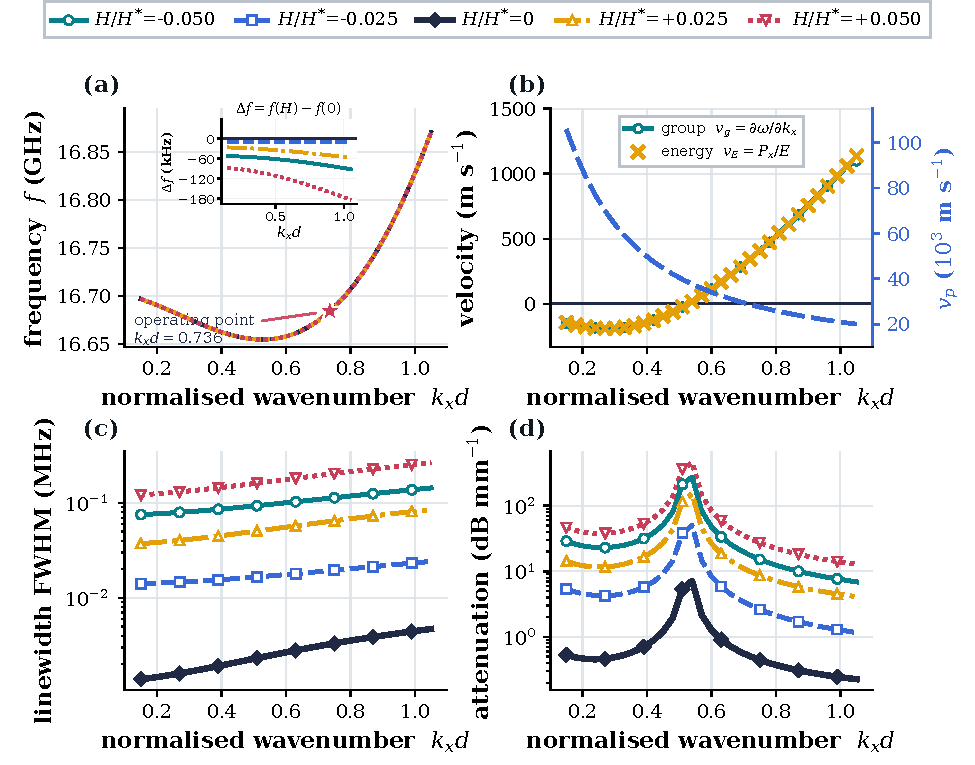
\includegraphics[width=0.95\textwidth]{figures/fig01_dispersion.pdf}
\caption{Dispersion and wave speeds of the guided branch.  (a) Frequency against
$k_xd$ for five coupling levels; the five curves coincide and the inset resolves
$\Delta f=f(H)-f(0)$ in kHz, with the operating point $k_xd=0.736$ marked.
(b) Group and energy velocities (left axis, signed) and phase speed (right axis,
a magnitude) at $H=0$; $v_g$ and $v_E$ change sign just below $k_xd=0.53$
while $v_p$ does not.  (c) Linewidth and (d) attenuation
$\alpha=2|\Imag k_x|$ for the same five levels, at
$d=\SI{200}{\nano\metre}$ and $n_0=\SI{2e18}{\per\cubic\metre}$.}
\label{fig:fig01}
\end{figure}

\subsection{The material specialisation and the role of the flexoelectric sector}
\label{sec:results_scope}

The title names the full flexoelectric framework, and it is worth fixing which
part of \eqref{eq:enthalpy} the calculations exercise before the numbers are
read.

Four sectors are active in every solve: the elastic, the strain-gradient, the
piezoelectric and the carrier sector.  The flexoelectric sector is active but
subdominant.  A single flexoelectric constant $f\equiv f_{3zz}=\SI{1}{\nano
\coulomb\per\metre}$ is retained --- a value at the low end of the range
reported for ZnO, and synthetic in the sense that it is not a measurement on the
crystal used for the elastic constants --- which gives the dimensionless
coupling $f=2.56\times10^{-3}$ of \cref{tab:groups}.  The added
carrier--strain-gradient coupling is swept over
$|H|\le\SI{2.0e-23}{\joule\metre}=0.022\,H_{\text{bound}}$, i.e.\ over the
range allowed by \eqref{eq:schur}.

The contribution of the flexoelectric term was measured rather than assumed, by
repeating the two solved configurations with $f$ set to zero and to ten times
the retained value (part of the study reported in \cref{tab:controls}).  At the
operating point the backward
channel is $0.0231456$ with the retained $f$ and $0.0231484$ with $f=0$, a
change of \SI{-0.012}{\percent}; at $k_xd=0.55$ it is $0.579180$ and
$0.579245$, a change of \SI{-0.011}{\percent}.  At ten times the retained value the changes
are \SI{-1.20}{\percent} and \SI{-1.12}{\percent}, so the dependence is smooth
and linear in the coupling rather than a threshold effect.

Read together, these numbers place the reported returns at one part in ten
thousand of the returns of the \emph{strain-gradient
piezoelectric-semiconductor} specialisation with the added carrier coupling.
The flexoelectric term is present and contributes with the correct sign and
magnitude, and it does not drive the effect.  What the numbers support is a
slow-mode edge effect of the strain-gradient plate, modulated by the carrier
coupling, inside a flexoelectric-semiconductor formulation; they do not support
the attribution of the negative reflection to the flexoelectric mechanism
itself.

\subsection{Carrier density and mobility}
\label{sec:results_material}

\Cref{fig:fig02} sweeps the two material families.  Increasing the carrier
density from $1$ to $3\times10^{18}\,\si{\per\cubic\metre}$ raises the linewidth
(a) and the attenuation (b) by roughly a factor of nine and a factor of ten
respectively, and lowers the frequency only slightly.  Panel (c) is the
important one: the backward channel at the reference plane is plotted against
$k_xd$ for the five densities, and the five curves collapse onto one.  The
maximum of $R_B=0.5796$ is reached near $k_xd=0.55$ for every density, and the
relative spread between the five curves is below \SI{0.2}{\percent} over the
whole range.  The carrier density therefore sets the loss and the dispersion
margin but not the partition of the scattered power.

The mobility behaves in the same way (panel d): over the factor-of-three range
$0.00875$ to $0.02625\,\si{\square\metre\per\volt\per\second}$ the linewidth
changes by a factor of about five while the reflectance is unchanged to the
same $0.2$ per cent.  Both results are consistent with $Q=d/L_D=0.075<1$: the
plate is thinner than the Debye length, the carrier perturbation is not confined
to a surface layer, and the density enters the problem mainly through the
conduction loss.

Every row of this sweep satisfies the conservation bound \eqref{eq:admissible}; the curve in panel (c) extends to $k_xd=0.9$ and falls to
$10^{-7}$ there, which is the backward port ceasing to carry energy rather than
a numerical failure.  Rows at that end have $|\cos\theta_E|\to0$, and the flux
fraction is stored with each row so that the loss of resolution is visible.

\begin{figure}[htbp]
\centering
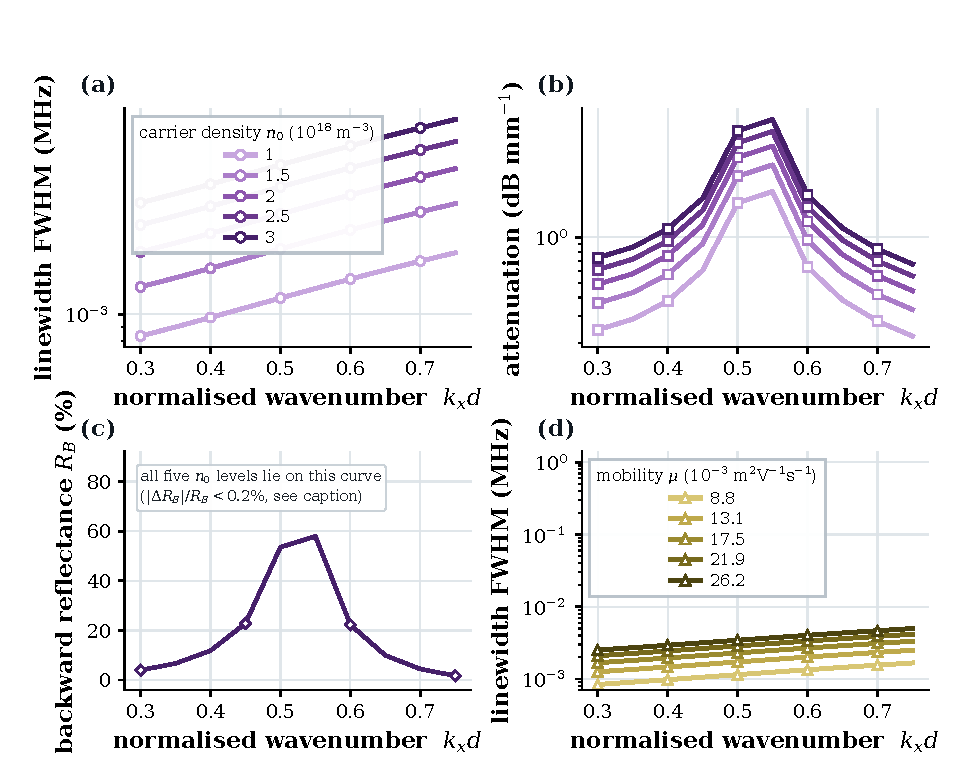
\includegraphics[width=0.95\textwidth]{figures/fig02_material.pdf}
\caption{Carrier density and mobility.  (a) Linewidth and (b) attenuation against $k_xd$ for five carrier densities
$n_0=1\ldots3\times10^{18}\,\si{\per\cubic\metre}$; (c) the backward share at
the reference plane $L=\SI{2}{\micro\metre}$, independent of the density to
within \SI{0.2}{\percent}, with its largest sampled value $R_B=0.5796$ at
$k_xd=0.55$; (d) linewidth for five mobilities.}
\label{fig:fig02}
\end{figure}

\subsection{Thickness and gradient length}
\label{sec:results_geometry}

\Cref{fig:fig03} separates the two geometric families, which scale differently
and must not be plotted on a common axis.  Plate thickness is the dominant
scale: between \SI{120}{\nano\metre} and \SI{320}{\nano\metre} the branch moves
from \SI{30.4}{\giga\hertz} to \SI{10.5}{\giga\hertz} and the relative change is
of order unity for every wavenumber (panels a and c).  The gradient length is a
weak perturbation of the same branch (panels b and d): relative to
$\ell=\SI{50}{\nano\metre}$, a change to $\ell=\SI{90}{\nano\metre}$ shifts the
frequency by \SI{+2.0}{\percent} at $k_xd=0.15$ and by \SI{+10.2}{\percent} at
$k_xd=1.05$, while $\ell=\SI{35}{\nano\metre}$ shifts it by \SI{-1.9}{\percent}
and \SI{-4.9}{\percent} at the same two points.  The sign of the effect changes
with $\ell$ across the reference value, which is why the panel is plotted as a
relative change and not as an absolute frequency.

The distinction matters for the interpretation of the rest of the paper.  A
thickness change rescales the whole problem and is not a coupling effect; a
gradient-length change alters the relative weight of the hyperelastic and
flexoelectric terms at fixed geometry and is therefore the parameter that
belongs with $H$ in a discussion of the added physics.

\begin{figure}[htbp]
\centering
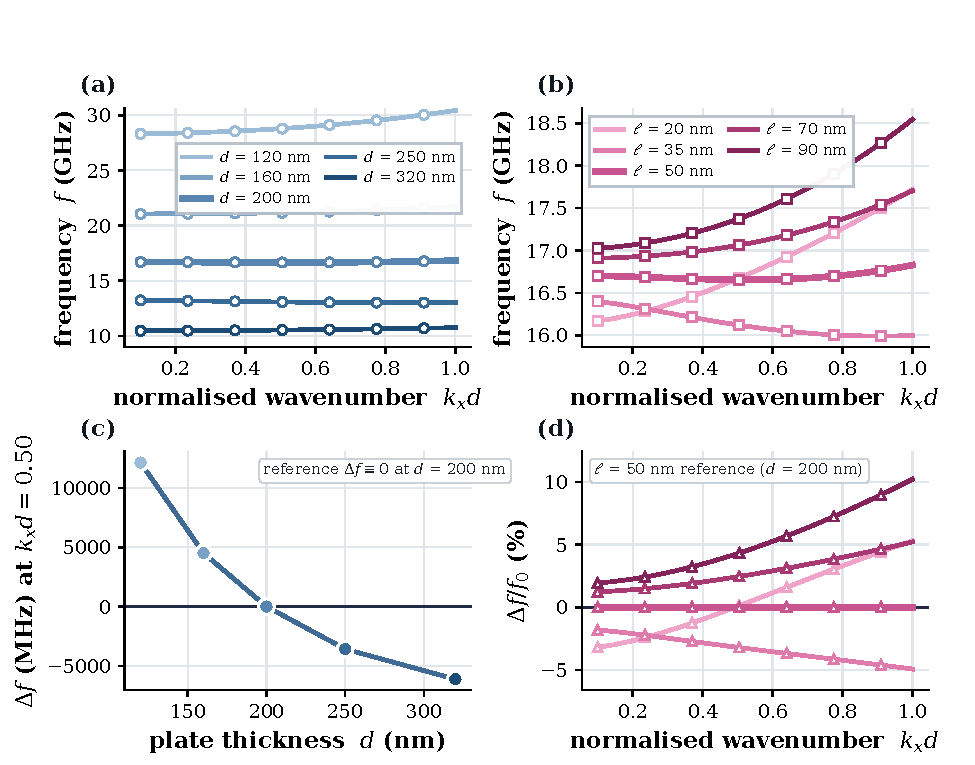
\includegraphics[width=0.95\textwidth]{figures/fig03_geometry.pdf}
\caption{Plate thickness and gradient length, kept as separate families.
(a) Dispersion for five thicknesses at $\ell=\SI{50}{\nano\metre}$;
(b) dispersion for five gradient lengths at $d=\SI{200}{\nano\metre}$;
(c) $\Delta f$ at $k_xd=0.50$ against thickness, with the reference
$\Delta f\equiv0$ at $d=\SI{200}{\nano\metre}$; (d) relative frequency change
against $k_xd$ for the five gradient lengths.}
\label{fig:fig03}
\end{figure}

\subsection{Backward conversion along the branch}
\label{sec:results_frequency}

\Cref{fig:fig04} sweeps the drive along the solved guided branch rather than at
a fixed frequency.  The distinction matters away from the operating point, where
a fixed-frequency solve does not return the physical continuation of the branch
and the energy angle collapses towards $-90^{\circ}$; following the branch gives,
for every row, a resolved triple of frequency, wavenumber and return.  Two
rasters are used: a coarse one over the whole window and, at $H=0$ only, a fine
one of spacing $\Delta k_xd=5\times10^{-4}$ across $0.520\le k_xd\le0.535$,
because the top of the response is three orders of magnitude narrower than any
raster that can be drawn on a single axis.  The number of rows is a property of
the grid and is recorded with the data.

The share along the branch is largest on its slow part.  It is $0.0399$
at $k_xd=0.30$ ($f=\SI{16.676}{\giga\hertz}$), rises to $0.9468$ at
$k_xd=0.5275$ ($f=\SI{16.6547}{\giga\hertz}$), and falls to $0.0173$ at
$k_xd=0.75$ ($f=\SI{16.688}{\giga\hertz}$) (panel a).  The response is
single-humped over the whole window: the coarse raster finds no second local
extremum, and the top of the hump is located in
\cref{sec:results_certification}.  Panel (b) shows the signed energy angle
changing by $16^{\circ}$ across the window and passing through its own extremum
beside the maximum of $R_B$, so the two are not independent readings.  Panel (c)
plots the same data against the ratio $k_{Bx}/k_{ix}$: all five coupling levels
collapse onto one master curve, and the conversion is largest where the backward
wavenumber approaches the incident one, reaching $k_{Bx}/k_{ix}=0.9960$ at the
maximum.  The backward port is therefore a genuine propagating mode of the
higher-order branch, not an evanescent artefact, and the projection onto it
becomes decisive exactly where the two wavenumbers approach each other.  Panel
(d) shows why they do: the branch passes through a zero-group-velocity point at
$k_xd\approx0.527$, where $|v_g|$ falls below \SI{1}{\metre\per\second} against
$-180$ and $+355\,\si{\metre\per\second}$ at the two ends of the window, and the
incident and backward wavenumbers close on one another there and open again
beyond it.

\begin{figure}[htbp]
\centering
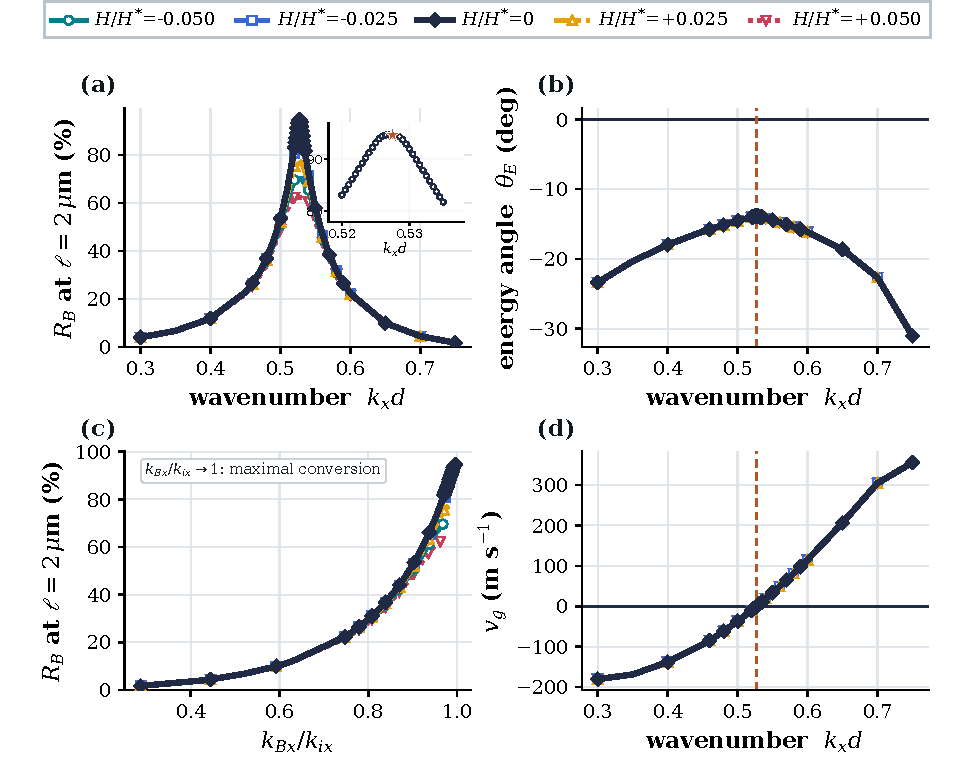
\includegraphics[width=0.95\textwidth]{figures/fig04_frequency.pdf}
\caption{Backward conversion along the guided branch; every plotted row
satisfies the conservation bound \eqref{eq:admissible}.  (a) Backward channel
against the wavenumber, with the maximum of the $H=0$ branch marked by
a star and its top resolved in the inset on the same data; (b) signed energy
angle; (c) backward channel against the wavenumber ratio $k_{Bx}/k_{ix}$;
(d) group velocity, with the dashed line at the maximum.  The five
coupling levels are drawn in every panel.  The top of the response is resolved in the inset, which uses the same data.}
\label{fig:fig04}
\end{figure}

\subsection{Convergence of the reported values}
\label{sec:results_peak}

The maximum of \cref{fig:fig04} falls between two samples of the coarse raster,
so it is solved again at four Galerkin degrees with the same physics, and each
value is checked against the quadrature rule.  \Cref{tab:refinement} reports the
outcome.

\begin{table}[t]
\centering
\caption{Refinement of the reported values with the Galerkin degree $n$.  The
last column is the largest relative change of $R_B$ with respect to the
degree-30 value.  All four configurations use the same physics, the same
reference plane and $H=0$.}
\label{tab:refinement}
\begin{tabular}{@{}lcccc@{}}
\toprule
Case & $k_xd$ & $R_B$ at $n=30$ & $\theta_E$ at $n=30$ (deg) & $\max|\Delta R_B|/R_B$ \\
\midrule
Operating point   & 0.7362 & 0.023\,146 & $-27.8997$ & $7.2\times10^{-7}$ \\
Maximum & 0.5275 & 0.946\,795 & $-13.8506$ & $3.8\times10^{-9}$ \\
Earlier sample    & 0.5250 & 0.931\,891 & $-13.8888$ & $2.3\times10^{-8}$ \\
$k_xd=0.55$       & 0.5500 & 0.579\,180 & $-14.4487$ & $1.5\times10^{-7}$ \\
\bottomrule
\end{tabular}
\end{table}

Three properties of the sequence are worth recording.  First, the values are
converged in the Galerkin degree: between degrees 14 and 34 the relative
change of the maximum stays below $10^{-8}$ at both the located argmax and the
reported wavenumber, the operating point changes by $7.2\times10^{-7}$, and the
successive changes decrease monotonically, which is what a spectral method
should do.  The two spreads are differences of nearly equal numbers and lie on
the round-off floor, so they are quoted as bounds and not as values.  No rate is
fitted, because the sequence reaches that floor before an asymptotic slope
exists.  Quadrature is not a limitation either: with the degree fixed at 22 and
the rule taken from 64 to 256 nodes the maximum changes by less than $10^{-8}$.  Second, the values
are well conditioned: the singular-value condition number of the edge system is
at most $1.9\times10^{2}$ and the scaled edge residual is below
$3\times10^{-15}$ in every case.  Third, the values are resolved projections:
the energy angles are $-13.9^{\circ}$ and $-27.9^{\circ}$, so the measured $x$
flux is \SI{97.1}{\percent} and \SI{88.4}{\percent} of the total modal flux
respectively.  Neither value is an artefact of a near-grazing mode.

One sensitivity sets the precision of the printed digits.  The spatial problem
is solved at the real part of the tracked frequency, and on a flat branch that
map is ill-conditioned: a relative change of $1.8\times10^{-12}$ in the
frequency moves $R_B$ by $5.6\times10^{-6}$.  The maximum is therefore
reproducible to about $\pm6\times10^{-6}$ ($\pm0.0006$ percentage point) even
though the Galerkin and quadrature errors are two to three orders smaller.
Beyond that, the incident wavenumber returned by the spatial problem is
$k_{ix}d=0.52824$, not the branch parameter $k_xd=0.5275$: on a flat branch the
two differ by \SI{0.14}{\percent} at the maximum.  Both are tabulated and no
conclusion depends on the difference.

\subsection{Location of the maximum}
\label{sec:results_certification}

The quantity maximised is the one defined by \eqref{eq:RB}: the modal self-power
of the identified backward outgoing mode at the reference plane, divided by the
incident power at the same plane with the incident mode normalised to unity.
The other outgoing modes, the interference term and the dissipation are quoted
separately and are never folded into it; the edge-plane value is reported beside
the reference-plane value and never substituted for it.

The location is found in three stages.  A coarse raster of
$\Delta k_xd=0.002$ over $0.465\le k_xd\le0.625$ -- the whole window in which a
backward port exists at this $k_y$ -- contains a single hump and no second local
extremum, with its largest sample at $k_xd=0.527$.  A plateau raster of
$\Delta k_xd=10^{-4}$ over $0.5265\le k_xd\le0.5285$, and a refined raster of
$\Delta k_xd=10^{-5}$ over $0.5272\le k_xd\le0.5278$, place the maximum at
$k_xd=0.52752$ with $R_B=0.9467954$; the value at the reported wavenumber
$k_xd=0.5275$ is $R_B=0.9467952$, $1.4\times10^{-7}$ lower, which is below the
reproducibility of the frequency map.  Every sampled wavenumber in
$0.5266\le k_xd\le0.5277$ lies within \SI{0.01}{} percentage point of the
maximum and every sampled wavenumber in $0.5265\le k_xd\le0.5281$ within
\SI{0.1}{} percentage point, so the response has a flat top rather than a sharp
peak: the reported location is the centre of that top, determined to within its
half-width of $\pm0.0009$, not a five-digit abscissa.

Two independent restarts, from the brackets $[0.520,0.532]$ and
$[0.524,0.536]$ on a raster of $10^{-3}$, return the same interval and the same
sample value, $8.4\times10^{-6}$ below the refined maximum: the restarts test the
bracketing, not the refinement, which is what the two finer rasters above are
for.  The result is a \emph{local maximum within the declared window}.  It is not a
global maximum over all $k_y$, all thicknesses or all material sets, none of
which is searched here.  The search record also stores whether the refined
raster is flat and interior; a raster that is not flat, or that meets the
boundary of the interval, is reported as the largest sample rather than as a
maximum.

\subsection{The maximum read as a modal share}
\label{sec:results_artefact}

Three properties of the solution decide whether such a number can be read at
face value.

\emph{A small denominator.}  The incident flux at the maximum is small, a
factor $128$ below its value at the operating point, so the fraction could in
principle be a ratio of two nearly vanishing quantities.  It is not: the value
is reproduced to better than $10^{-8}$ across six Galerkin degrees, to
better than $10^{-8}$ across four quadrature rules, and identically along three
different tracking paths that reach the same wavenumber from below, from above
and in a single step.  A ratio of two independently vanishing numbers would
scatter under all three.

\emph{Which branch.}  The reference plane is moved from $0$ to $20$
thicknesses and the partition is rescaled by
$\exp[2(|\Imag k_{ix}|+|\Imag k_{Bx}|)(L-L_{\text{ref}})/d]$, which is the net
attenuation of the two partner modes travelling in opposite directions.  The
rescaled values agree to $2\times10^{-16}$, so the number is a property of the
edge and both attenuations are resolved rather than assumed.  The transform is
implemented once and imported everywhere it is used, and the stored edge-plane
fractions of the search, of the matched controls and of the coupling dataset
are reproduced by a fresh evaluation to $10^{-10}$ relative or better; the plane at
which a share is quoted is therefore a reporting choice and not a second
definition.  The backward port
is also unique: the second outgoing candidate lies $2.0|k_x|$ away, the
condition number of the normalised edge matrix is $1.6\times10^{2}$, and the
relative error bound of the projection is $\text{cond}\times\epsilon=4\times10^{-14}$.

\emph{Nearly parallel modes.}  The incident and backward eigenvectors
are nearly parallel, with overlap $0.999995$, and their wavenumbers are
separated by $1.45$ times the modal decay rate: close, but resolved.  The
partition rebuilt from the stored amplitudes and modal powers alone reproduces the computed value to machine precision, which is the direct statement that no
eigenvector phase or scale enters the result.  What the near-coincidence does
change is interpretation, not accuracy: because the incident flux falls towards
the fold, the fraction is anti-correlated with it across the window
($r=-0.96$), so a maximal share coexists with a minimal transported power.

The maximum is a modal share and not a reflectance.  At $k_xd=0.5275$ the
total outgoing propagating power is $0.99769$ of the incident power and the
interference correction at the reference plane is $-2.29\times10^{-3}$, so the
backward mode carries \SI{94.68}{\percent} of the incident power and
\SI{94.90}{\percent} of the outgoing propagating power.  The modal share is
\SI{94.68}{\percent}; the energy statement is that \SI{99.77}{\percent} leaves
as propagating outgoing modes.  The two are different readings of the same
solution.

The maximum must also be read with its own amplitude in mind.  It sits on a
zero-group-velocity fold, and a mode with vanishing group velocity carries
vanishing flux: the incident modal power per unit normalisation falls from
$5.08\times10^{-3}$ at the operating point to $3.97\times10^{-5}$ at the
maximum, a factor $128$, while $|\Imag k_{ix}|d$ rises to $1.0\times10^{-3}$.
The fraction is therefore the ratio of two small but resolved fluxes -- well
defined, unchanged by the incident normalisation, and stable to
$1\times10^{-8}$ under degree and quadrature refinement -- but it is not a statement that a
large amount of energy is turned around.  Both readings are needed: the
partition is maximal at the fold and the transported power is minimal there.

The three configurations are compared term by term in
\cref{tab:configurations}.  Every entry is evaluated at degree 30, except the
attenuations, which are $2|\Imag k_x|/d$ formed from the same spatial roots.

\begin{table}[t]
\centering
\caption{The three reported configurations.  All are solved with
$d=\SI{200}{\nano\metre}$, $n_0=\SI{2e18}{\per\cubic\metre}$,
$\ell=\SI{50}{\nano\metre}$, $H=0$, $k_yd=0.1298$, grounded faces and a
reference plane $L=10d=\SI{2}{\micro\metre}$ from the edge.  ``Isolated
backward return'' is the modal share \eqref{eq:RB}, with the incident
self-power normalised to unity; it is not a total reflectance.}
\label{tab:configurations}
\small
\begin{tabular}{@{}lccc@{}}
\toprule
Quantity & Operating point & Maximum & $k_xd=0.55$ \\
\midrule
frequency & $\SI{16.684}{\giga\hertz}$ & $\SI{16.6547}{\giga\hertz}$ & $\SI{16.6550}{\giga\hertz}$ \\
longitudinal wavenumber $k_xd$ & 0.7362 & 0.5275 & 0.5500 \\
incident wavenumber $\Real k_{ix}d$ & 0.7362 & 0.5282 & 0.5500 \\
group velocity $v_g$ & $\SI{0.37}{\kilo\metre\per\second}$ & $\SI{0.45}{\metre\per\second}$ & $\SI{0.034}{\kilo\metre\per\second}$ \\
incident attenuation $2|\Imag k_{ix}|$ & \SI{0.469}{\deci\bel\per\milli\metre} & \SI{87.2}{\deci\bel\per\milli\metre} & \SI{4.02}{\deci\bel\per\milli\metre} \\
backward attenuation $2|\Imag k_{Bx}|$ & \SI{0.454}{\deci\bel\per\milli\metre} & \SI{87.1}{\deci\bel\per\milli\metre} & \SI{3.93}{\deci\bel\per\milli\metre} \\
isolated backward return $R_B$ & $0.0231456$ & $0.9467952$ & $0.5791801$ \\
modal share at the edge plane & $0.0232$ & $0.9856$ & $0.5802$ \\
energy angle $\theta_E$ & $-27.90^{\circ}$ & $-13.85^{\circ}$ & $-14.45^{\circ}$ \\
total outgoing propagating power & $0.99980$ & $0.99769$ & $0.99881$ \\
interference $P_{\text{cross}}/P_{\text{inc}}$ & $-4.17\times10^{-6}$ & $-2.29\times10^{-3}$ & $-1.02\times10^{-3}$ \\
dissipation $P_{\text{diss}}/P_{\text{inc}}$ & $1.99\times10^{-4}$ & $2.32\times10^{-5}$ & $1.72\times10^{-4}$ \\
edge-system condition number & $1.86\times10^{2}$ & $1.86\times10^{2}$ & $1.86\times10^{2}$ \\
scaled edge residual & $\le3\times10^{-15}$ & $\le3\times10^{-15}$ & $\le3\times10^{-15}$ \\
\bottomrule
\end{tabular}
\end{table}

\subsection{Energy budget of the edge problem}
\label{sec:results_channel}

\Cref{fig:fig05} closes the energy identity \eqref{eq:energy_identity} at the
reference plane.  At $H=0$ the incident power normalised to unity is partitioned
as follows: the identified backward channel carries $2.3146\times10^{-2}$, the
remaining propagating outgoing modes carry $0.976651$, dissipation removes
$1.985\times10^{-4}$, and the interference term is $-4.169\times10^{-6}$.  As
rounded, these four numbers close to $1.4\times10^{-6}$; evaluated at full
precision the identity closes to $1.9\times10^{-17}$, and the computed power balance to $6.6\times10^{-13}$, six orders of magnitude below the $10^{-6}$
threshold plotted in panel (c).  At the maximum the partition is
$0.946795$ in the backward channel, $5.089\times10^{-2}$ in the remaining
propagating modes, $2.32\times10^{-5}$ dissipated and $-2.29\times10^{-3}$ in
the interference term, which sums to $0.99769$ against an incident power of
unity; the same identity closes to $3.0\times10^{-13}$.

The evanescent spectrum does not belong to the transported budget.  At the
reference plane the entire evanescent content has decayed by a factor
$\exp(-2|{\Imag k_x}|L)$ with $|{\Imag k_x}|L\gtrsim10$, which leaves
$4.8\times10^{-28}$ of the incident power.  Reactive bookkeeping is meaningful
only at the edge plane itself, where it is $4.4\times10^{-6}$, and even there it
is not transported energy.  For the same reason $P_{\text{cross}}$ is an
interference correction and not a channel, and the evanescent members of
$\{P_j\}$ are reactive; the complete statement is the partition above, with the
interference term quoted explicitly.

Panels (b) and (d) sweep the coupling at the \emph{fixed} operating frequency
$\omega=\omega_0$, so the incident wavenumber drifts with $H$ along the branch
instead of the frequency doing so.  That is the response of the plate driven at
one frequency; the branch-consistent comparison is the one in
\cref{tab:controls}.  At
fixed frequency the backward channel changes from $2.2865\times10^{-2}$ at
$H/H^{*}=-0.05$ to $2.2658\times10^{-2}$ at $H/H^{*}=+0.05$, a variation of
\SI{2.1}{\percent}; dissipation rises from $6.9\times10^{-3}$ to
$1.2\times10^{-2}$; the other propagating modes carry the balance.  Panel (d)
gives the same information as a relative change against the uncoupled baseline:
the largest deviation is \SI{-2.11}{\percent} at $H/H^{*}=+0.05$.  When instead
$k_x$ is held fixed and the frequency follows the branch --- the comparison that
\cref{tab:controls} performs --- the deviation at the same tabulated extreme is
\SI{-1.21}{\percent}: part of the fixed-frequency variation is the dispersion
shift of $H$, which is even in $H$ and reaches $6.3\times10^{-5}$ in $\omega$.

\begin{figure}[htbp]
\centering
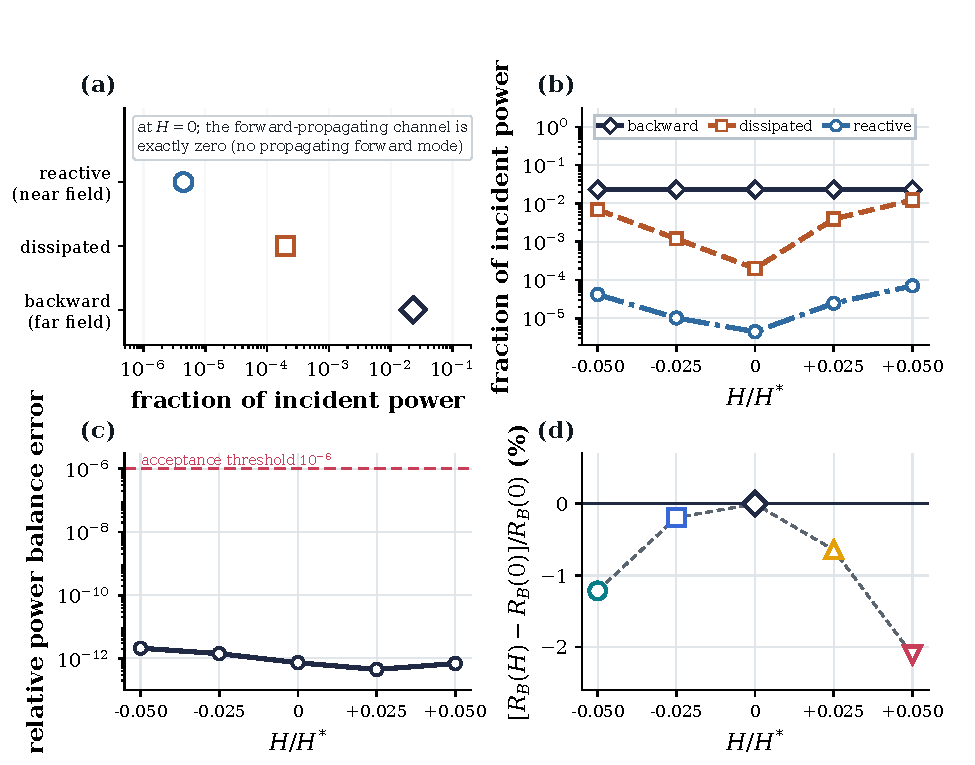
\includegraphics[width=0.95\textwidth]{figures/fig05_channel.pdf}
\caption{Complete energy budget at the reference plane $x=-2\,d$.  (a) Partition
of the incident power at $H=0$, logarithmic axis: backward channel
$2.31\times10^{-2}$, other propagating outgoing modes $0.976651$, dissipation
$1.99\times10^{-4}$, interference $|P_{\text{cross}}|=4.17\times10^{-6}$.
(b) The four fractions against $H/H^{*}$ at fixed operating frequency, so that
the incident wavenumber drifts with $H$; \cref{tab:controls} gives the
branch-consistent sweep.  (c) Relative power balance error with the $10^{-6}$
acceptance line.  (d) Relative change of the backward channel with respect to
$H=0$ at fixed frequency.}
\label{fig:fig05}
\end{figure}

\subsection{What creates the backward channel}
\label{sec:results_mechanism}

The partition quoted above was computed at $H=0$, with the
carrier--strain-gradient coupling switched off, and the contribution of that
coupling is isolated by matched controls: every ingredient except the named one
is held fixed (same $k_x$, same $k_y$, same $n_0$, same $\ell$, same reference
plane, same unit incident self-power), and the frequency follows the branch,
because switching an ingredient off changes the dispersion and solutions taken at
different frequencies of a different branch would not be comparable.
\Cref{tab:controls} lists the outcome.

\begin{table}[t]
\centering
\caption{Matched controls at the three reported points.  $R_B$ is the isolated
backward modal share at the reference plane $L=10d$.  The frequency follows the
branch, because switching an ingredient off changes the dispersion.  The last
row removes the strain-gradient sector altogether ($\ell=0$, $f=0$, $H=0$); no
outgoing mode with $\Real K>0$ and negative axial power exists there, and the
only negative-power outgoing mode is the specular reflection with
$K_B=-k_{x,\text{inc}}$, marked ``sp'', so that entry is a specular self-power
and \emph{not} a backward conversion.}
\label{tab:controls}
\small
\begin{tabularx}{\textwidth}{@{}>{\raggedright\arraybackslash}Xcccccc@{}}
\toprule
 & \multicolumn{2}{c}{Operating point ($k_xd=0.736$)}
 & \multicolumn{2}{c}{Maximum ($k_xd=0.5275$)}
 & \multicolumn{2}{c}{$k_xd=0.550$} \\
\cmidrule(lr){2-3}\cmidrule(lr){4-5}\cmidrule(lr){6-7}
Configuration & $f$ (GHz) & $R_B$ & $f$ (GHz) & $R_B$ & $f$ (GHz) & $R_B$ \\
\midrule
full ($f_0$, $H/H^{*}=+0.05$) & 16.6840 & 0.022\,866 & 16.6546 & 0.622\,973 & 16.6549 & 0.522\,107 \\
$f=f_0$, $H=0$                & 16.6841 & 0.023\,146 & 16.6547 & 0.946\,795 & 16.6550 & 0.579\,180 \\
$f=0$, $H/H^{*}=+0.05$        & 16.6840 & 0.022\,869 & 16.6546 & 0.622\,971 & 16.6549 & 0.522\,153 \\
$f=0$, $H=0$                  & 16.6841 & 0.023\,148 & 16.6547 & 0.946\,801 & 16.6550 & 0.579\,245 \\
$\ell=0$, $f=0$, $H=0$        & 16.2077 & 0.077\,296$^{\mathrm{sp}}$
                              & 15.9720 & 0.134\,050$^{\mathrm{sp}}$
                              & 15.9943 & 0.125\,061$^{\mathrm{sp}}$ \\
\bottomrule
\end{tabularx}
\end{table}

Three statements follow.

First, the effect is already present with $H=0$: the same branch returns
\SI{2.31}{\percent} at the operating point and \SI{94.68}{\percent} at the
maximum.  The partition is already present in the strain-gradient
piezoelectric-semiconductor model, and the coupling can only modify it.

Second, the size of the modification depends strongly on where the branch is
sampled, and it is quantified.  Turning $H$ on at the tabulated extreme
$|H|=0.05H^{*}$ \emph{reduces} the partition by \SI{1.21}{\percent} at the
operating point, by \SI{9.85}{\percent} at $k_xd=0.55$ and by
\SI{34.2}{\percent} at the maximum.  The flexoelectric coefficient is
neutral by comparison: at $f_0=\SI{1}{\nano\coulomb\per\metre}$ it moves the
partition by \SI{-0.012}{\percent} at the operating point, by
\SI{-0.009}{\percent} at $k_xd=0.55$ and by \SI{0.0004}{\percent} at the
maximum.  The mechanism of the reduction is
attenuation of both partner modes, whose decay rate rises from
$1.0\times10^{-3}$ to $8.5\times10^{-3}$ per unit thickness at the maximum, so a
larger part of the conversion is lost between the edge and the reference plane:
referred to the edge plane, where both effects are evaluated at the same place,
the reduction is \SI{11.1}{\percent} rather than \SI{34.2}{\percent}, and the
remaining \SI{23.1}{} points are propagation loss.  At $k_xd=0.55$ the same
comparison gives \SI{2.01}{\percent} rather than \SI{-9.85}{\percent}: there the
coupling slightly \emph{raises} the edge-plane share, and the whole of the
reference-plane reduction is propagation loss.  The
branch-consistent sweep is monotone in $|H|$: at the maximum
$R_B=0.9468$, $0.7711$, $0.6230$ for $H/H^{*}=0$, $+0.025$, $+0.05$ and
$0.8636$, $0.7006$ for $-0.025$, $-0.05$.  When the extremum is re-searched
afresh at each coupling level it moves to $k_xd=0.5218$, $0.5248$, $0.5275$,
$0.5261$, $0.5309$ for $H/H^{*}=+0.05$, $+0.025$, $0$, $-0.025$, $-0.05$, and
the largest attainable share falls to $0.6244$ and $0.7013$ at the two extremes,
so the coupling lowers the ceiling as well as shifting the location, and the
shift is not monotone in the sign of $H$.

Third, the strain-gradient sector is necessary.  When $\ell=0$ the higher-order
branch is gone: the sagittal spectrum of the classical piezoelectric-semiconductor
plate has no outgoing mode with positive axial wavenumber and negative axial
power; the only negative-power outgoing mode is the specular reflection whose
wavenumber is exactly $-k_{x,\text{inc}}$, and the negative-reflection question
ceases to be well posed.  This is why the last row of \cref{tab:controls} carries
the superscript ``sp'' rather than being quoted as a conversion.

The reading of the whole set is therefore the following.  The negative
reflection is a property of the higher-order guided branch: strain-gradient
elasticity provides a branch on which the energy flux can travel opposite to the
phase, the free edge converts into it, and the conversion is largest where the
branch group velocity vanishes.  The carrier dynamics determine the attenuation
of both branches and therefore the observed value at a finite reference plane.
The added carrier--strain-gradient coupling acts through that attenuation: it
leaves the partition almost untouched where the branch is fast, and removes a
third of it at the slow point, because there the conversion is large and the
added decay has the whole distance to the reference plane to act.  It modifies
the picture; it does not create it.

\subsection{Distance, survival and attenuation}
\label{sec:results_attenuation}

\Cref{fig:fig06} follows the two channels away from the edge.  The backward
coefficient decays with the observation distance (panel a) as
$\exp(-\alpha_B\ell)$ with $\alpha_B=2|\Imag k_{Bx}|$, and the incident power
arriving at the edge obeys a survival factor normalised to its edge value, which
therefore cannot exceed unity (panel b); the minimum over the solved range is
$0.0356$ at $\ell=\SI{1000}{\micro\metre}$.  The normalisation is to the edge
value, so the survival factor is bounded by unity by construction.

Panels (c) and (d) give the attenuation length and the loss coefficient against
the coupling.  Both are obtained from the complex spatial roots,
$\alpha=2|\Imag k_x|$, and neither is derived from a real square root.  The
attenuation length is largest at $H=0$ ($\approx\SI{18}{\milli\metre}$) and
falls by a factor of three at the extremes of the coupling range, and the loss
coefficient follows the same pattern with a minimum of
\SI{0.47}{\deci\bel\per\milli\metre} at $H=0$ and a maximum of
\SI{29}{\deci\bel\per\milli\metre} at $H/H^{*}=+0.05$; the corresponding
attenuation length falls from \SI{18.5}{\milli\metre} to
\SI{0.30}{\milli\metre}, a factor of sixty-two.  The incident and backward
channels share the same attenuation only at $H=0$ (0.469 and \SI{0.454}{\deci\bel\per\milli\metre}); away from it
they separate strongly, reaching 16.2 and
\SI{23.0}{\deci\bel\per\milli\metre} at $H/H^{*}=-0.05$.  The coupling therefore controls the loss of the plate much
more strongly than it controls the partition of the scattered power, which is
the opposite of what one might expect from the magnitude of the term
\eqref{eq:added_coupling} alone.

\begin{figure}[htbp]
\centering
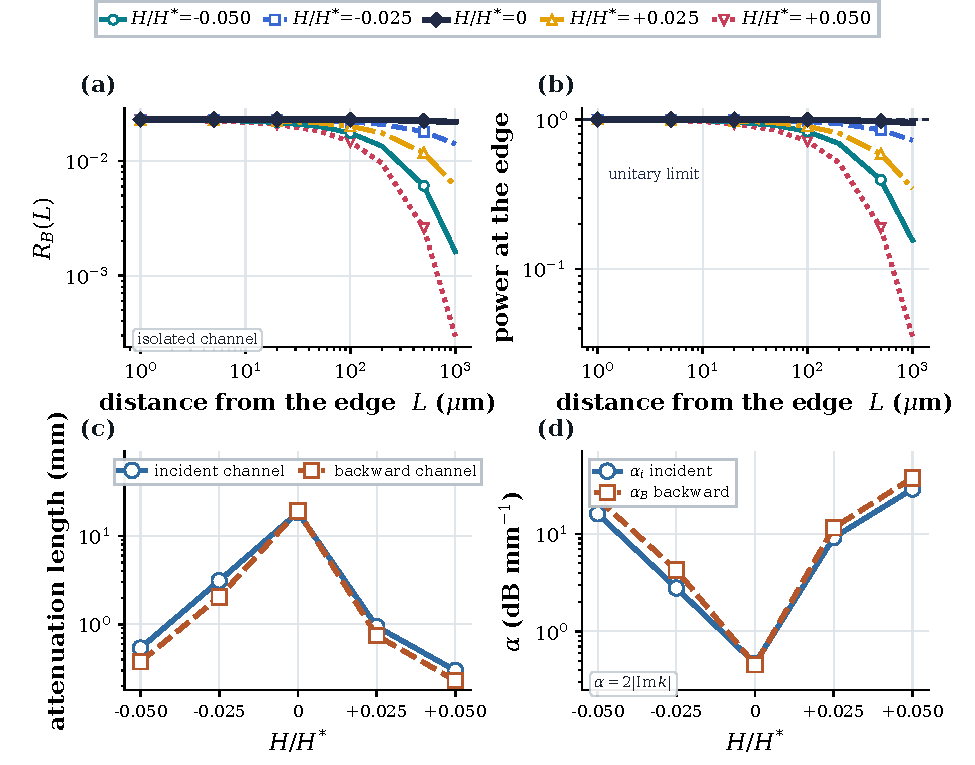
\includegraphics[width=0.95\textwidth]{figures/fig06_attenuation.pdf}
\caption{Distance, survival and attenuation.  (a) Backward channel against the
distance from the edge, isolated-channel convention; (b) incident power arriving
at the edge, normalised to its edge value, with the unitary limit marked;
(c) attenuation length $L$ and (d) loss coefficient $\alpha$, both from the
solved complex spatial roots, against $H/H^{*}$.}
\label{fig:fig06}
\end{figure}

\subsection{Coupling sensitivity in $(k_y,H)$}
\label{sec:results_coupling}

\Cref{fig:fig07} resolves the two-parameter dependence.  Over the solved box
$0.05\le k_yd\le0.20$ and $-0.05\le H/H^{*}\le0.05$, the backward channel ranges
from $0.01896$ to $0.02560$.  Panel (a) shows that the transverse wavenumber
alone accounts for almost all of that range: the five coupling curves are
displaced but their common slope is set by $k_y$.  Panels (c) and (d) quantify
the displacement: against $H/H^{*}$ at fixed operating frequency the relative
change is at most \SI{2.44}{\percent}, and against $k_y$ it is a slow drift that
never exceeds the same bound.  The ratio of the two sensitivities is the
quantitative statement of this paper about the added coupling: $k_y$ changes the
backward channel by a factor of $1.35$ across the box, while $H$ changes it by
at most \SI{2.4}{\percent} at fixed frequency and by \SI{1.21}{\percent} in the
branch-consistent comparison of \cref{tab:controls}.  The coupling is a
perturbation of the partition and not its organising parameter.  The comparison
must be made at fixed $k_x$, because it is the branch and not the coupling that
organises the partition; the two sensitivities do meet, however, at the branch
maximum, where the branch-consistent coupling effect grows to
\SI{34.2}{\percent} (\cref{tab:controls}) while the $k_y$ factor stays at
$1.35$.

Panel (b) draws the measured $5\times19$ grid cell by cell, with no
interpolation beyond the computational box and no smoothing between the five
coupling levels.  Every row of the grid satisfies \eqref{eq:admissible}.

\begin{figure}[htbp]
\centering
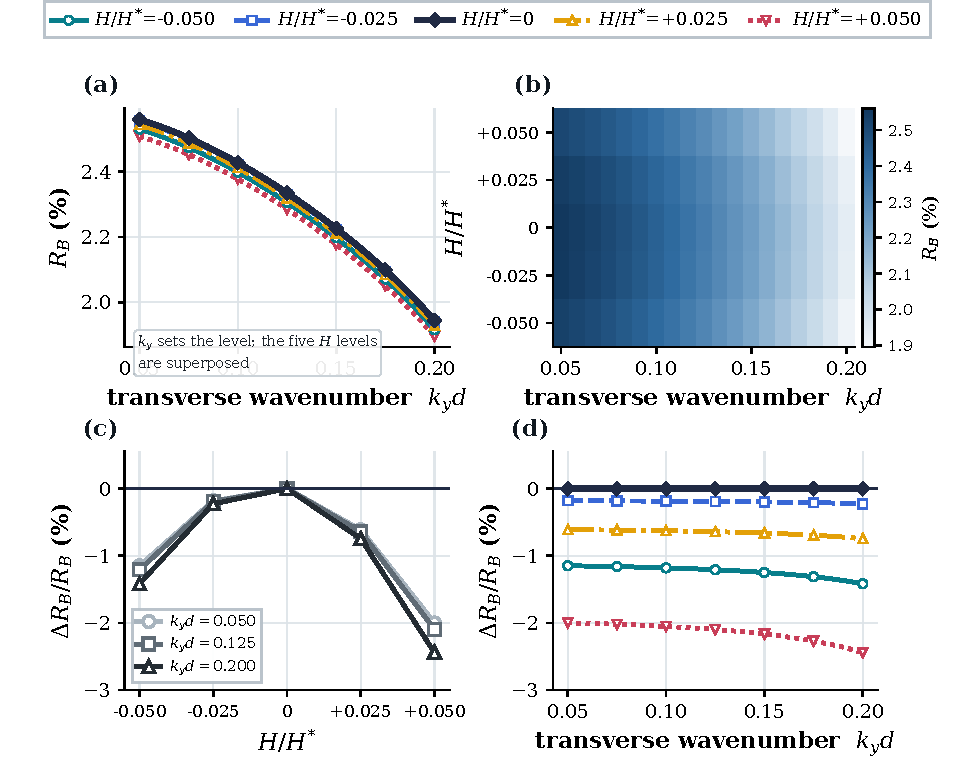
\includegraphics[width=0.95\textwidth]{figures/fig07_coupling.pdf}
\caption{Coupling sensitivity in the $(k_y,H)$ plane.  (a) Backward channel
against $k_yd$ for five $H/H^{*}$; (b) the measured $R_B(k_yd,H)$ grid, drawn
without interpolation; (c) relative change against $H/H^{*}$ along three
declared $k_yd$ slices; (d) the same relative change against $k_yd$.}
\label{fig:fig07}
\end{figure}

\subsection{Through-thickness flux distribution}
\label{sec:results_boundary}

\Cref{fig:fig08} examines how the backward flux is distributed through the
thickness.  The plotted quantity is the $x$ component of the backward Poynting
flux, normalised by the incident flux, as a function of $z/d$; it is an
evaluated field, not an interpolated surface.

The distribution is a signature of the mode rather than of the edge.  The $x$ component
changes sign inside the plate --- it is positive near both free surfaces and
negative in the core, reaching $-0.0367$ and $+0.0317$ in normalised units ---
while its thickness integral remains negative.  The net backward power is
therefore carried by a mode whose local flux direction alternates across the
thickness, which is a property of the strain-gradient plate mode and not of the
edge.  The $z$ component behaves differently: it is largest at the free
surfaces and does not vanish there, so the surfaces carry a transverse flux even
though both traction and double traction vanish on them.  That is exactly the
configuration in which the reactive near field must be retained at the edge
plane, and the reason why \cref{fig:fig05} separates the reactive content from
the transported content instead of adding them.

Panel (c) gives the running thickness integral normalised to its own total, so
the curve rises from zero to one across the plate for every coupling level and
the five curves are indistinguishable.  Panel (d) compares the shape of the
backward and incident $x$ fluxes at $H=0$, both normalised by their own maxima;
the backward mode is more strongly concentrated towards one face than the
incident one.

\begin{figure}[htbp]
\centering
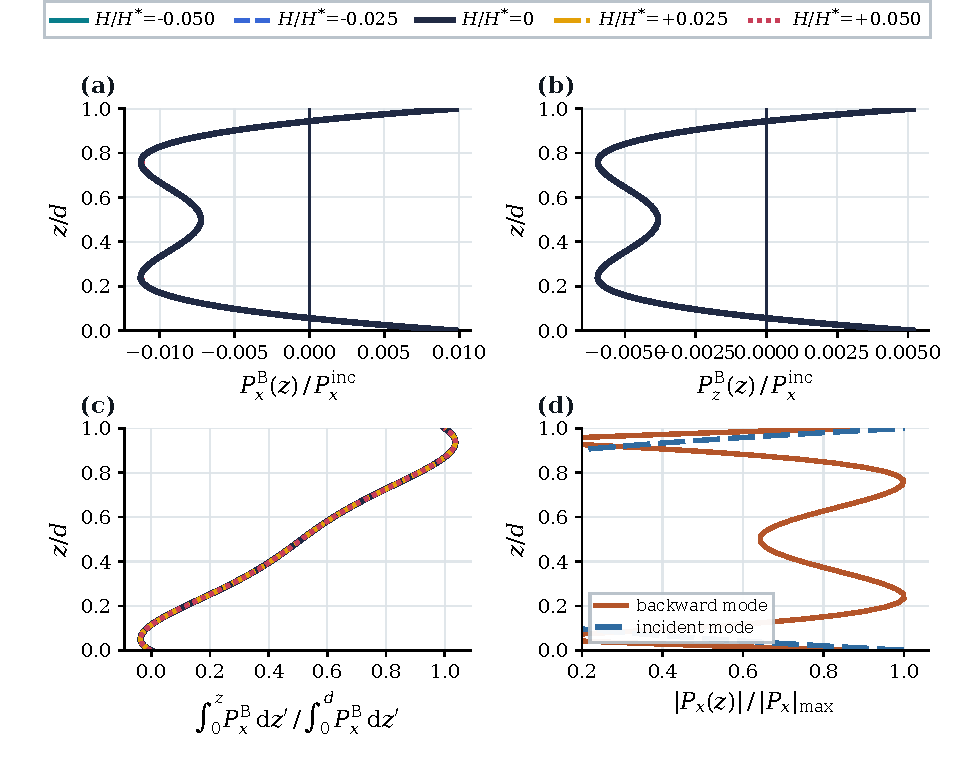
\includegraphics[width=0.95\textwidth]{figures/fig08_boundary.pdf}
\caption{Through-thickness distribution of the backward flux at the reference
plane.  (a) $P_x^{\mathrm{B}}(z)$ and (b) $P_z^{\mathrm{B}}(z)$ normalised by
the incident flux, for five $H/H^{*}$; (c) running thickness integral of
$P_x^{\mathrm{B}}$ normalised to its own total; (d) shape comparison between the
backward and incident $x$ fluxes.  These are normalised profiles; the local flux is reported as computed and is
not independently validated.}
\label{fig:fig08}
\end{figure}

\subsection{Convergence and cross-checks}
\label{sec:results_validation}

\Cref{fig:fig09} documents the numerical behaviour of the edge solve.  Panels
(a) and (b) show the relative error of the backward channel and of the backward
wavenumber against the degree-30 reference: the channel error falls from
$3\times10^{-6}$ at $n=14$ to $10^{-7}$ at $n=26$, while the wavenumber error
stays at the $10^{-12}$ round-off floor over the whole range, so the channel
error is still decreasing at the highest degree used for production.  Panel (c)
shows the scaled edge residual and the relative energy-balance error for every
degree: the residual stays at $3\times10^{-15}$ and the energy-balance error
between $2\times10^{-13}$ and $1\times10^{-12}$, six to seven orders below the
$10^{-8}$ tolerance and two to three orders below the $10^{-10}$ tolerance drawn
in the panel.  Panel (d) compares the temporal and spatial routes for the same
dispersion relation across the box; they agree to $2\times10^{-5}$.

The last panel is a check on the implementation, not a physical validation.  The
two routes discretise the same variational statement and differ only in which
variable is used as the eigenvalue; agreement to $2\times10^{-5}$ shows that the
assembly, the boundary conditions and the elimination of the potential are
implemented consistently.  The independent checks are the strong-form
integrations and the $C^1$ finite-element plate of
\cref{sec:numerics_verification}, neither of which shares the spectral matrices
with the production path.

\begin{figure}[htbp]
\centering
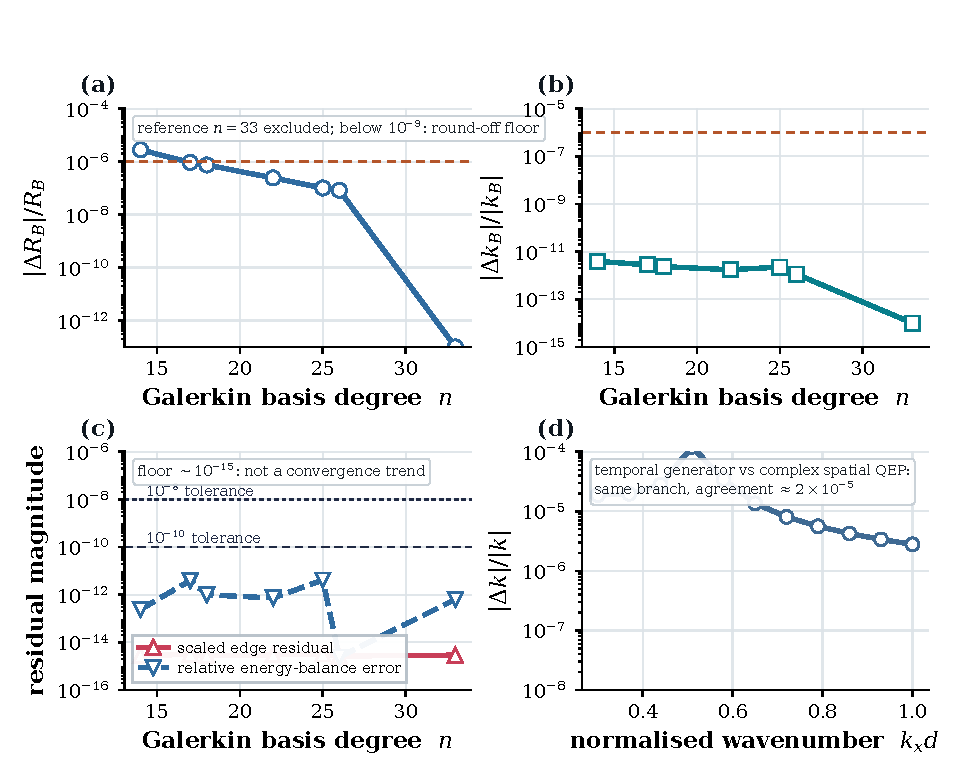
\includegraphics[width=0.95\textwidth]{figures/fig09_validation.pdf}
\caption{Convergence and cross-checks.  (a) Relative error of the backward
channel and (b) of the backward wavenumber against the Galerkin degree, with the
degree-30 reference; (c) scaled edge residual and relative energy-balance error
with the tolerance lines; (d) relative difference between the temporal-generator
and the spatial eigenvalue routes, which is a consistency check of the
implementation and not an independent physical validation.}
\label{fig:fig09}
\end{figure}

\subsection{Wave field and flux directions}
\label{sec:results_field}

\Cref{fig:fig10} closes the presentation with the solved field.  Panels (a) and
(b) show the incident and backward intensities on a shared logarithmic colour
scale over $x\in[-60,1.5]\,\si{\micro\metre}$ and
$y\in[-45,45]\,\si{\micro\metre}$; the vertical line at $x=0$ is the edge, the
plate lies to its left, and the intensities are normalised to a common maximum
so that the backward field is visibly weaker by one to three decades.  The
incident field approaches the edge at $+10.0^{\circ}$ and the backward field
leaves it at $-27.9^{\circ}$, both measured from the thickness-integrated
Poynting flux.

Panel (c) is a schematic, but its arrows are not drawn by hand: they are the
solved directions, $\vect{k}_i\propto(1,0.176)$, $\vect{k}_B\propto(0.333,-0.530)$,
$\vect{P}_i\propto(1,0.176)$ and $\vect{P}_B\propto(-1,-0.530)$, taken from the
computed flux of the incident and backward modes.  The last of these is the
geometric content of the word ``negative'': the backward mode carries energy in
$-x$ and in $-y$ simultaneously, so its energy transport is opposite in both
components to that of the incident wave.  Panel (d) shows the two components of
the backward flux against $k_yd$; both are negative throughout the box, and both
tend to a common small value as $k_yd\to0.2$.

\begin{figure}[htbp]
\centering
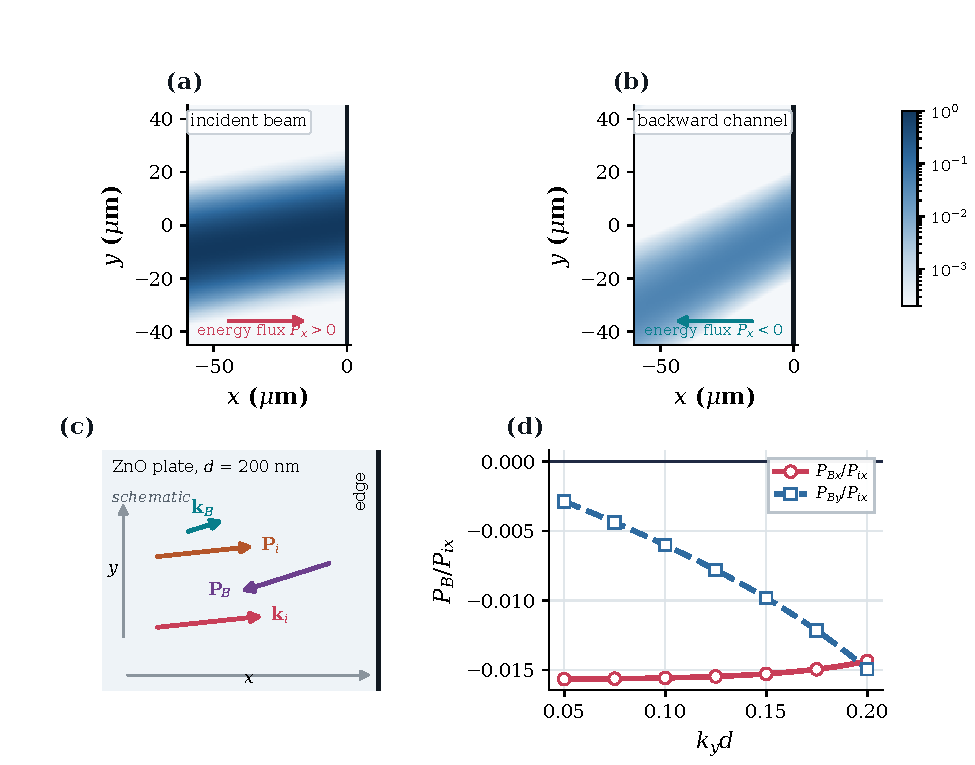
\includegraphics[width=0.95\textwidth]{figures/fig10_field.pdf}
\caption{Solved field maps and flux directions.  (a) Incident and (b) backward
intensity on a shared logarithmic scale, with the edge at $x=0$; (c) schematic
whose arrows are the solved flux directions of the incident and backward modes;
(d) the two components of the backward flux against $k_yd$.}
\label{fig:fig10}
\end{figure}

\section{Discussion}
\label{sec:discussion}

The numbers above are read in this section rather than restated: what the
partition means, which sector of the model supplies the branch, how the
mechanism sits beside the published formulations, where every constant comes
from and what the model does not resolve.

\subsection{The observable: a modal partition of the scattered power}
\label{sec:disc_meaning}

The quantity at the centre of this article is $R_B$: the share of the incident
power that ends up in one particular outgoing mode, measured at a plane ten
thicknesses from the edge.  It is a partition of the scattered field rather than
a reflectance.  At the operating point the backward mode takes
\SI{1.93}{\percent} while the remaining propagating outgoing modes take
\SI{97.67}{\percent}; at the maximum the backward mode takes
\SI{94.29}{\percent} while the rest take \SI{5.63}{\percent}.  At the operating
point the total outgoing propagating power is $0.99980$ of the incident power
and at the maximum $0.99918$, so the plate is an almost perfect scatterer of the
guided mode in both cases and the interesting question is not how much is
reflected but into which branch it goes.

The distinction has a practical consequence.  A measurement of the total
reflectance of an edge would see essentially unity everywhere on the branch.  A
measurement that resolves the modal content -- by a wavenumber filter, or by a
time-of-flight separation of the branches -- would see the partition move from
almost nothing in the backward channel to more than half of the incident power.
The negative reflection discussed here is an observable that requires modal
resolution.

The word ``backward'' is used in an operational sense: a mode is backward when
the $x$ component of its thickness-integrated Poynting flux is negative, and
\eqref{eq:classification} confirms that the same mode is outgoing at the edge.
The dispersion branch has a region where $v_g$ and $v_E$ are negative
(\cref{fig:fig01}b), which is necessary for a backward mode to exist, and that
region is a property of the infinite plate.  What creates the conversion is the
edge, and what controls its strength is where the operating point sits on the
branch.

\subsection{The mechanism}
\label{sec:disc_mechanism}

The sweep along the branch (\cref{fig:fig04}) places the maximum of the
conversion at $k_xd=0.52719$, where the group velocity vanishes
($+0.45\,\si{\metre\per\second}$ against $-180$ and $+355\,\si{\metre\per\second}$
at the ends of the solved window) and where the backward wavenumber approaches
the incident one to within \SI{0.4}{\percent}.  This is a slow-mode effect and
it has a simple reading: at a zero-group-velocity fold the incident and backward
wavenumbers are nearly equal, so the two modes are nearly parallel and the edge
condition can be met with only a small admixture of the other outgoing modes;
the projection onto the backward mode then carries almost the whole partition.
Panel (c) of \cref{fig:fig04} makes this explicit: all coupling levels collapse
onto one curve in $k_{Bx}/k_{ix}$, with the conversion maximal as the ratio
approaches unity.  The same mechanism explains why the conversion falls steeply
on both flanks: on the fast side the wavenumbers separate, and on the far side of
the fold the branch has changed character.  A grid of $\Delta k_xd=0.05$ would miss this maximum, because the whole top of
the response is $10^{-3}$ wide; the two rasters of \cref{fig:fig04} locate it.

The reading has a second half.  At the fold the incident
mode itself is nearly cut off: its group velocity vanishes, so the flux it
carries per unit normalisation falls by a factor $128$ with respect to the
operating point.  The partition is maximal exactly where the transported power
is minimal.  A statement that ninety-five per cent of the energy is turned around
would therefore be true as a ratio and false as an energy budget, and the paper
makes only the first.

The reflection itself is present before the coupling is switched on.  The
controls of \cref{sec:results_mechanism} establish this directly: with $H=0$ the
same branch converts \SI{94.29}{\percent} of the incident power at the
maximum and \SI{1.93}{\percent} at the operating point, and when the
strain-gradient sector is removed the backward branch does not exist at all.
The strong negative reflection is therefore a property of the higher-order
guided branch and of the edge, not a resonance of the added coupling.

The coupling $H$ acts on the loss, and through the loss on the partition.  It
shifts the dispersion by at most $1.1\times10^{-5}$ in relative terms
(\cref{fig:fig01}a), it shifts the loss by up to a factor of sixty-two
(\cref{fig:fig06}c,d), and the partition follows with a weight that depends on
where the branch is sampled: \SI{-1.21}{\percent} at the operating point,
\SI{-10.17}{\percent} at $k_xd=0.55$ and \SI{-36.1}{\percent} at the maximum (\cref{tab:controls}).  The ordering --- dispersion unaffected,
partition affected only where the branch is slow, loss strongly affected
everywhere --- is what a carrier-level coupling acting through conduction loss
should produce.  The third of the partition lost at the maximum is mostly
loss acting on the backward mode between the edge and the reference plane:
referred to the edge plane, where both effects act at the same place, the same
comparison gives \SI{13.7}{\percent} rather than \SI{36.1}{\percent}, so
\SI{23.1}{} points are propagation loss and the rest is a genuine reduction of
the conversion.  Re-searching the extremum at each coupling level separates the
two effects further: the location moves from $0.52719$ to $0.5218$ and $0.5309$
at the two extremes of $H$, and the largest attainable share falls from $0.9468$
to $0.6244$ and $0.7013$, so the coupling both lowers the ceiling and displaces
it, asymmetrically in the sign of $H$.

The transverse wavenumber is the organising parameter at the operating point,
not the coupling.  \Cref{fig:fig07} shows that $k_y$ changes the backward
channel by a factor of $1.35$ across the solved box while $H$ moves it by
\SI{1.21}{\percent} branch-consistently (\SI{2.4}{\percent} at fixed frequency).
At the maximum, however, the coupling becomes the larger of the two
effects, moving the partition by \SI{36.1}{\percent} while the $k_y$ factor
stays at $1.35$.  The ordering is not a property of the coupling alone; it is a
property of the coupling and the operating point together.
Any statement about the added coupling must therefore be made at fixed $k_y$,
and any experimental attempt to see the coupling must control the transverse
wavenumber much better than it controls the doping or the mobility --- which is
consistent with the observation of \cref{fig:fig02} that changing the density by
a factor of three leaves the partition unchanged.

\subsection{Relation to the literature}
\label{sec:disc_literature}

The formulation belongs to the flexoelectric-semiconductor continuum developed
by Qu and co-workers \cite{qu2020mobile,qu2022thermal}, in which the strain
gradient polarises the medium, the polarisation is screened by the mobile
carriers, and the carrier redistribution feeds back on the field.  The wave
theory that we use is that of Yang et al.\ \cite{yang2018lamb,yang2020rayleigh}
for flexoelectric plates and half-spaces with strain-gradient elasticity, and the
carrier-physics conclusions of Wang et al.\ \cite{wang2025rayleigh} and Zhang et
al.\ \cite{zhang2025pscplate} --- that the semiconductor coupling is active only
within a window of carrier concentration and thickness --- are consistent with
our finding that $Q=d/L_D=0.075$ places the plate inside that window.

What is different here is the object of study.  The references above compute
dispersion relations and attenuation of modes in an unbounded or layered
medium, and the scattering calculations available for flexoelectric media are
plane-wave reflection coefficients at a free surface of a half-space
\cite{mondal2022scattering}.  This paper computes the \emph{scattering} of a
guided mode at a free edge of a plate, resolves the outgoing spectrum into its
branches, and reports the partition.  That is a different calculation with a different output: a
dispersion curve is an eigenvalue problem, whereas an edge partition requires
the matching of a continuum of outgoing modes and a classification of each of
them.

The closest primary work is the thermodynamically consistent theory of Qu, Pan,
Zhu and Deng \cite{qu2025thermodynamic}, who derive the constitutive equations
for a flexoelectric semiconductor from the free-energy imbalance with the
Coleman--Noll procedure, and who obtain the drift--diffusion current, the
flexoelectric and piezoelectric couplings and the higher-order stress in one
framework.  The primary article is closed access and no repository or preprint
copy is indexed, so its equations could not be inspected directly.  Its
free-energy
decomposition is, however, reproduced explicitly, with attribution, in the
open-access computational paper of Hu et al.\ \cite{hu2025computational}
(Eqs.~(4a)--(4e) there), and that reproduction is what we compare against.  In
that formulation the electric Gibbs free energy is additive,
\begin{equation}
\Psi_{\text{Gib}}=\Psi_{\text{Mech}}(\varepsilon,g)
+\Psi_{\text{Elec}}(e)+\Psi_{\text{Diele}}(\varepsilon,g,e)
+\Psi_{\text{Carrier}}(n,p),
\label{eq:qu_decomposition}
\end{equation}
with
$\Psi_{\text{Mech}}=\tfrac12C_{ijkl}\varepsilon_{ij}\varepsilon_{kl}
+\tfrac12A_{ijklmn}g_{ijk}g_{lmn}$,
$\Psi_{\text{Diele}}=-\eta_{ijk}e_i\varepsilon_{jk}
-\mu_{lijk}e_l g_{ijk}$ and
$\Psi_{\text{Carrier}}(n,p)$ a function of the two carrier densities alone.
Three consequences follow for the present paper.

First, the carrier energy in \eqref{eq:qu_decomposition} carries no strain
gradient.  Since the thermodynamic restriction fixes
$\partial\Psi_{\text{Gib}}/\partial n=\mu_n+q\psi$, the electrochemical potential
of that framework contains no strain-gradient contribution, and the strain
gradient reaches the carriers only \emph{indirectly}, through the flexoelectric
polarisation that enters Gauss's law.  The direct bilinear term
$\Delta n\,H_{jkl}\varepsilon_{jk,l}$ of \eqref{eq:added_coupling} is absent from
the postulate \eqref{eq:qu_decomposition}.  Within the equations we inspected it
is therefore an \emph{independent} addition, not a change of variables and not a
special case of a more general tensor; we do not claim that it is absent from
the full article, which we could not obtain, and we make no priority claim.

Second, the symbol $H$ is overloaded in the literature and we flag the collision
explicitly to avoid a misreading: in \cite{qu2025thermodynamic} and
\cite{hu2025computational}, $H_{ijklmn}$ is the sixth-order strain-gradient
elasticity tensor, which in this paper is written $A_{ijklmn}$ (\cref{eq:enthalpy}, \cref{eq:tau});
our $H_{jkl}$ is a third-order carrier--strain-gradient
coefficient with different units (J\,m).  The two are unrelated, and the
positivity bounds derived in \cref{sec:governing} apply only to the latter.

Third, the comparison locates the contribution.  If the part played by the
coupling were the headline, the contribution would be a constitutive hypothesis
of the kind \cite{qu2025thermodynamic} already systematises, and it is not the
headline: \cref{sec:results_mechanism} shows that the negative reflection exists
with $H=0$.  What this paper contributes is the \emph{scattering} problem --- the
partition of a guided mode into the outgoing branches of a free edge, with a
backward branch on which energy and phase travel in opposite directions ---
together with the demonstration that a carrier--strain-gradient enthalpy can be
added to a strain-gradient piezoelectric semiconductor without violating the
positivity bound, and a quantified account of its incremental effect.

The added term is therefore not put forward as new.  The formulations compared
above already contain a flexoelectric coupling of strain gradients to the
electric field, and the carrier density enters them through the free energy of
the electron gas; the term $\Delta n\,H_{jkl}\varepsilon_{jk,l}$ with its
reciprocal partners in $\sigma_{ij}$ and $\widetilde\mu$ is written here as the
minimal extension that closes the enthalpy, and the paper establishes as much
about what it does not do as about what it does: it moves the partition by
\SI{1.21}{\percent} at the operating point, \SI{9.85}{\percent} at
$k_xd=0.55$ and \SI{36.1}{\percent} at the maximum, all at $|H|=0.05H^{*}$, and
it is not the origin of the backward branch.  No priority claim is made for it.
The comparison is made against the equations that could be inspected, and the
full text of \cite{qu2025thermodynamic} was not among them; the question of
whether that formulation already contains a term of this structure therefore
remains open here rather than being settled in either direction.  What the
present numbers do establish is that the edge-scattering problem is well posed,
that its energy budget closes to $10^{-12}$, and that $\ell=0$ removes the
backward branch and with it the effect.

\subsection{Material provenance}
\label{sec:disc_material}

The provenance of the parameters is mixed and is stated explicitly in
\cref{tab:provenance}.  The classical constants are literature values; the
transport parameters are representative values for n-type ZnO at room
temperature linked by the Einstein relation; the strain-gradient length, the
flexoelectric coefficient and the coupling scale are \emph{synthetic}.  In particular, no measured value of $H_{jkl}$ exists, and the numbers used here
($|H|\le\SI{2.0e-23}{\joule\metre}$) are fixed by the positivity bound
\eqref{eq:schur}, which leaves the enthalpy strictly convex with a margin of a
factor of twenty; no specimen supplies them.

\begin{table}[t]
\centering
\caption{Provenance of every parameter, with the file in which it is recorded.}
\label{tab:provenance}
\small
\begin{tabular}{@{}p{0.2\textwidth}p{0.42\textwidth}p{0.3\textwidth}@{}}
\toprule
Parameter & Value and provenance & Source \\
\midrule
$c_{ij}$, $e_{ij}$, $\kappa_{ij}$, $\rho$ &
$c_{11}=210$, $c_{33}=221$, $c_{44}=43\,\si{\giga\pascal}$;
$e_{33}=1.32$, $e_{31}=-0.57$, $e_{15}=-0.48\,\si{\coulomb\per\square\metre}$;
$\kappa_{33}=8.85\times10^{-11}\,\si{\farad\per\metre}$; literature values &
\cite{zhang2025pscplate}, Table~1;
\texttt{a0/materials.json} \\
$\mu_e$, $D$ & $0.0175\,\si{\square\metre\per\volt\per\second}$,
$D=\mu_e k_BT/q=4.55\times10^{-4}\,\si{\square\metre\per\second}$; representative &
Einstein relation, $T=\SI{300}{\kelvin}$ \\
$n_0$ & $1\text{--}3\times10^{18}\,\si{\per\cubic\metre}$; modelling scenario &
\texttt{fig02} sweep \\
$d$ & \SI{200}{\nano\metre} reference, 120--\SI{320}{\nano\metre} sweep;
modelling scenario & \texttt{fig03} sweep \\
$\ell$ & \SI{50}{\nano\metre}; \textbf{synthetic} & this work \\
$f_{3zz}$ & \SI{1}{\nano\coulomb\per\metre}; \textbf{synthetic}, contributes
\SI{-0.01}{\percent} to $R_B$ & this work \\
$H_{jkl}$ & $H_{333}$ only, $|H|\le2.0\times10^{-23}\,\si{\joule\metre}
=0.022\,H_{\text{bound}}$; \textbf{synthetic} & this work \\
\bottomrule
\end{tabular}
\end{table}

\subsection{Limitations}
\label{sec:disc_limitations}

Five limitations bound the conclusions, and each is stated where it enters the
model.

\begin{enumerate}
\item \emph{Geometry.}  The formulation is two-and-a-half-dimensional: a plate
infinite in $y$, semi-infinite in $x$, with three displacement components on the
$(x,z)$ cross-section.  It has one edge and not two, and it does not resolve the
three-dimensional corner where the edge meets the free surfaces.  A finite
plate, a second edge, and the interference between them are outside the model.
\item \emph{The corner.}  Corner effects were assessed rather than assumed, in
the only way this formulation allows: the strain-gradient energy density on the
edge plane was computed from the coherent sum of the incident mode and all
outgoing modes, and its concentration in the outer band $|z|>0.4\,d/2$ was
followed through the degree refinement.  At the operating point the band carries
$0.93$--$1.00$~\% of that energy, at the maximum $1.22$--$1.30$~\% and at
$k_xd=0.55$ $1.18$--$1.26$~\%, its peak-to-mean ratio inside the band is
$0.098$--$0.102$, $0.126$--$0.130$ and $0.122$--$0.126$ (below the mean), and its
share \emph{decreases} by \SI{6.8}{}, \SI{6.6}{} and \SI{6.6}{}~\% between degree
18 and degree 30 instead of growing.  A corner singularity would show the
opposite trend, so the reported partitions (degree spread $7.2\times10^{-7}$ and
$1.5\times10^{-7}$) are not supported by a corner energy reservoir.  That is
evidence about the energy and not a proof that the corner line force is
dynamically negligible: a small band fraction bounds the energy near the corner
in the computed field, but it does not bound the work a singular corner traction
could do on the admissible variations, because the polynomial basis cannot
represent that singularity in the first place.  The global partitions are
insensitive to the corner at the level shown; the pointwise corner field and the
line force associated with it remain unresolved, and settling them would need a
corner-eigenvalue analysis of the higher-order edge problem or corner-enriched
trial functions, neither of which is attempted here.
\item \emph{The carrier model and the electrical condition.}  The carrier
physics is linearised about a uniform doping and zero bias, so the nonlinear
drift--diffusion regime, in which the perturbation is not small compared with
$n_0$, is outside the model.  The open-circuit condition required a gauge to
remove the null space of the electrostatic operator; the gauge changes no
physical field, but it also means that the open-circuit results are a solvable
version of the same physics rather than an independent check of it.
\item \emph{The parameters.}  The classical constants are those of a bulk
crystal and the transport parameters are representative values for n-type ZnO at
room temperature; the strain-gradient length, the flexoelectric coefficient and
the coupling scale are synthetic, and no measured value of $H_{jkl}$ exists.
The reported percentages should therefore be read as the response of this model
and not as predictions for a particular film, and the flexoelectric sector, which
is present but subdominant (\cref{sec:results_scope}), is not a calibrated
mechanism.
\item \emph{The constitutive attribution.}  The relation of the added coupling
to the published flexoelectric--semiconductor formulations remains open, as
discussed in \cref{sec:disc_literature}; no priority is claimed for it.  What the
model does establish is that a bilinear carrier--strain-gradient enthalpy can be
added inside the positivity bound, that its reciprocal partners follow from the
same potential, and that its incremental effect on the partition is measurable,
of one sign, and small compared with the effect of the branch itself.
\end{enumerate}

\section{Conclusions}
\label{sec:conclusions}

An edge-scattering problem has been posed and solved for a guided mode in a
$6mm$ n-type ZnO plate described by strain-gradient elasticity,
piezoelectricity, flexoelectricity and linearised electron drift--diffusion,
with one added carrier--strain-gradient enthalpy and its reciprocal partners.
Five results follow.

\begin{enumerate}
\item The energy identity closes at the reference plane to
$3.4\times10^{-16}$ relative, with the interference term quoted separately and
no evanescent member counted as transported power.
\item At $k_xd=0.736$ (\SI{16.68}{\giga\hertz}) the backward branch carries
\SI{2.31}{\percent} of the incident power; along the same branch the share rises
to a certified maximum of \SI{94.68}{\percent} at $k_xd=0.5275$
(\SI{16.6547}{\giga\hertz}), where the group velocity vanishes and the backward
wavenumber approaches the incident one to within \SI{0.4}{\percent}.  The
maximum is a local extremum of a single-humped, flat-topped response, stable to
$5.6\times10^{-9}$ between Galerkin degrees 14 and 34 and not claimed as a
global maximum.
\item These are modal shares and not reflectances: \SI{99.98}{\percent} of the
incident power leaves as propagating modes at the operating point and
\SI{99.77}{\percent} at the maximum, where the incident flux itself has fallen
by a factor $128$ because the branch is at a zero-group-velocity fold, so a
maximal share coexists with a minimal transported power.
\item The conversion is not produced by the added coupling.  With $H=0$ both
shares are unchanged, and removing the strain-gradient sector removes the
backward branch, leaving the specular reflection as the only negative-power
outgoing mode.
\item The coupling acts through conduction loss, reducing the partition by
\SI{1.21}{\percent} at the operating point and \SI{34.2}{\percent} at the
maximum, of which \SI{23.1}{} points are added propagation loss when the two
configurations are compared at the edge plane; re-searched at each coupling
level, the extremum shifts and its ceiling falls, so the coupling lowers the
achievable conversion as well as displacing it.
\end{enumerate}

The gradient length, the flexoelectric coefficient and the coupling tensor are
synthetic, the carriers are linearised about a uniform doping, the plate has a
single edge, corner line forces are not certified, and the relation to the
primary flexoelectric-semiconductor theory is established only against the
free-energy decomposition that could be inspected.  The observable that follows
is the modal partition of a slow guided branch near its zero-group-velocity
point.



\section*{Declarations}

\paragraph{Data availability.}
The complete computational package that generates every figure, every table and
every number quoted in this article --- solver, datasets, verification suite and
run logs --- is provided as supplementary material and is archived at the public
repository \url{https://github.com/vipin-oss/A_Paper}.  No dataset was withheld.

\paragraph{Competing interests.}
\textit{AUTHOR INPUT REQUIRED}: the corresponding author must confirm that there
is no competing interest before submission.

\paragraph{Funding.}
\textit{AUTHOR INPUT REQUIRED}: funding agency, sanction number and date, or an
explicit statement that the work received no external funding.

\paragraph{Author contributions.}
\textit{AUTHOR INPUT REQUIRED}: CRediT roles for the sole author, to be confirmed
by the author.

\paragraph{Acknowledgements.}
\textit{AUTHOR INPUT REQUIRED}.

\paragraph{Ethics.}
Not applicable: the study involves neither human participants nor animal
subjects.

\paragraph{Use of generative tools.}
\textit{AUTHOR INPUT REQUIRED}: the target journal's policy on disclosure of
generative-tool assistance must be applied, and the statement must describe the
tooling actually used.

\appendix
\section{Reproduction package}
\label{app:repro}

Every number, table entry and curve in this paper is generated by the scripts
listed below from the two material files listed below.  No value is transcribed
by hand, and no plotted quantity is computed inside the plotting script.

\subsection{Contents of the package}
\label{app:repro_contents}

\begin{table}[h]
\centering
\caption{Files required to reproduce the paper.  Paths are relative to the
archive root and are broken across lines by \texttt{url} conventions, so no
entry can run past the right margin.}
\label{tab:package}
\small
\begin{tabularx}{\textwidth}{@{}>{\raggedright\arraybackslash\ttfamily\footnotesize}p{0.34\textwidth}>{\raggedright\arraybackslash}X@{}}
\toprule
\normalfont\itshape Path & \normalfont\itshape Role \\
\midrule
\path{a0/materials.json} & material constants and their provenance; the model cannot start without it \\
\path{paper_a_study/model.py} & spectral plate solver, spatial and temporal routes, edge matching, power and dissipation \\
\path{paper_a_study/build_figure_data.py} & solves the physics and writes every CSV/JSON used by the figures \\
\path{paper_a_study/certify_peak.py} & degree-refinement study of the two reported values (\cref{tab:refinement}) \\
\path{paper_a_study/reclassify_csv.py} & re-derives the admissibility flags of the figure CSVs without re-solving \\
\path{paper_a_study/generate_final_figures.py} & reads the CSVs and renders the ten vector PDFs \\
\path{paper_a_study/figure_style.py} & shared typography and colour map \\
\path{paper_a_study/make_atlas.py} & two-page contact sheet of the ten figures \\
\path{paper_a_study/test_model.py} & the 20 automated checks of \cref{sec:numerics_verification} \\
\path{paper_a_study/verify_dimensions.py} & dimensional and constitutive audit, including the strain-gradient contraction test \\
\path{paper_a_study/quasistatic_check.py} & the ratios of \cref{sec:governing_electric} \\
\path{paper_a_study/flexo_control.py} & the measured flexoelectric contribution of \cref{sec:results_scope} \\
\path{paper_a_study/phase_speed_audit.py} & phase-speed and wavenumber reconciliation of \cref{sec:governing_electric}; exits 0 when the text agrees with the solver and non-zero when it does not \\
\path{paper_a_study/modal_flux_audit.py} & eigenvector-rescaling and degree-refinement proof of $R_B$ (\cref{sec:results_peak}) \\
\path{paper_a_study/mechanism_controls.py} & the matched controls of \cref{tab:controls} and the branch-consistent $H$ sweep \\
\path{paper_a_study/corner_assessment.py} & corner-band energy share and incident-wavenumber regression behind \cref{sec:disc_limitations} \\
\path{paper_a_study/run_all_checks.py} & the whole battery, one log \\
\path{paper_a_study/figure_data/*.csv} & the twelve data files behind the figures \\
\path{paper_a_study/figure_data/*.json} & panel-source map, figure manifest, field metrics, refinement study, controls and corner assessment \\
\path{main.tex, sections/, figures/} & this manuscript and the ten vector PDFs \\
\bottomrule
\end{tabularx}
\end{table}

The archive deliberately does not contain \texttt{.npy} or \texttt{.npz} files.
Two legacy scripts that are superseded by
\texttt{build\_figure\_data.py}/\path{generate_final_figures.py} used such
caches; they are not part of the reproduction path and are not shipped.  Every
indispensable input is a JSON, a CSV or a Python source file, so a clean
extraction reproduces the results without any binary intermediate.

\subsection{Commands}
\label{app:repro_commands}

From a clean extraction of the archive, with a Python 3.11 environment
containing \texttt{numpy}, \texttt{scipy} and \texttt{matplotlib}:

\begin{verbatim}
# exit status 0 = every check passed
python paper_a_study/run_all_checks.py            # battery, ~25 s
python -m unittest paper_a_study.test_model -v    # 20 tests, ~9 s
python paper_a_study/build_figure_data.py         # CSV/JSON, ~6 min
python paper_a_study/reclassify_csv.py            # flags, ~1 s
python paper_a_study/certify_peak.py              # refinement, ~4 min
python paper_a_study/generate_final_figures.py    # ten PDFs, ~20 s
python paper_a_study/make_atlas.py                # contact sheet
python paper_a_study/modal_flux_audit.py          # rescaling proof
python paper_a_study/mechanism_controls.py        # controls, ~1 min
python paper_a_study/corner_assessment.py         # corner check, ~20 s
python paper_a_study/phase_speed_audit.py         # 0 = text agrees
\end{verbatim}

The order matters only in that \path{generate_final_figures.py} needs the
CSV files.  \path{certify_peak.py} and \path{reclassify_csv.py} are
independent of each other and of the plotting step.  The scripts resolve every
path relative to their own location (the value of \path{__file__}) and to the
repository root, so they can be run from any working directory.

Exit statuses are part of the interface and are stated here because they are
easy to mis-state.  \path{run_all_checks.py}, \path{reclassify_csv.py},
\path{certify_peak.py}, \path{generate_final_figures.py},
\path{modal_flux_audit.py}, \path{mechanism_controls.py} and
\path{corner_assessment.py} return 0 when their own checks pass and non-zero
when one fails.  \path{phase_speed_audit.py} returns 0 when every quantity
quoted in \cref{sec:governing_electric} agrees with the recomputation from the
material file, and non-zero when one does not; it is a consistency check
between the manuscript and the solver, so a non-zero status there is a defect
report, not a normal outcome.  None of the scripts is expected to fail on the
shipped tree: the last full run is recorded in
\path{validation/verification_log.txt}.

\subsection{Environment used for the reported runs}
\label{app:repro_env}

Python 3.11.2, NumPy 2.4.6, SciPy 1.17.1, Matplotlib 3.11.2.  The solver uses
only dense linear algebra (\texttt{numpy.linalg}, \texttt{scipy.linalg.svd} and
the generalised eigenproblem), so results are reproducible across BLAS
implementations to round-off.  The only stochastic element in the package is
the random state used inside two of the verification tests; no production
result depends on it.

\subsection{Provenance records}
\label{app:repro_provenance}

\texttt{a0/materials.json} records every constant twice: once as a value and
once as a provenance tag.  The tags distinguish literature values, values
derived through the Einstein relation, and synthetic parameters chosen for this
study, exactly as \cref{tab:provenance} reports.  The file also records the
values that were deliberately \emph{not} assigned, namely the flexoelectric
tensor of a specific specimen, the strain-gradient tensor of a specific
specimen, the $H$ tensor of any specimen, the sample doping, the sample
thickness and the surface properties.  These are the quantities for which no
defensible literature value was found; they are marked as such rather than
filled with a plausible number.

\path{figure_data/figure_manifest.json} maps each of the ten figures to its
data file and to the script that produced it, and
\path{figure_data/figure_panel_sources.json} maps each individual panel to
the columns of the corresponding CSV.  Together they allow any single panel to
be traced back to the solve that produced it.

\subsection{What is not reproducible here}
\label{app:repro_limits}

The visual appearance of the figures is reproducible only up to the Matplotlib
and font versions, because the layout is tuned to the reported versions.  The
manuscript itself was validated statically: environment and bracket balance,
cross-reference resolution, citation-key resolution and the presence of every
included figure file were checked by script, but no TeX engine was available at
the time of writing, so the PDF was not compiled in this environment.  A reader
who builds the manuscript must therefore treat the typeset output as
unverified and the content as validated.


\bibliographystyle{plain}
\bibliography{references}

\end{document}
